% Created 2024-04-25 Πεμ 21:04
% Intended LaTeX compiler: pdflatex
\documentclass[11pt]{article}
\usepackage[utf8]{inputenc}
\usepackage[T1]{fontenc}
\usepackage{graphicx}
\usepackage{longtable}
\usepackage{wrapfig}
\usepackage{rotating}
\usepackage[normalem]{ulem}
\usepackage{amsmath}
\usepackage{amssymb}
\usepackage{capt-of}
\usepackage{hyperref}
\usepackage{minted}
\usepackage[margin=2cm]{geometry}
\usepackage{setspace}
\usepackage{caption}
\usepackage{subcaption}
\usepackage{graphicx}
\graphicspath{{figures/}}
\usepackage{array}
\usepackage[utf8]{inputenc}
\usepackage[LGR]{fontenc}
\usepackage{csquotes}
\usepackage[T1]{fontenc}
\usepackage[english, greek, ]{babel}
\newcommand{\en}[1]{\selectlanguage{english}\text{#1}\selectlanguage{greek}}
\usepackage{minted}
\hypersetup{colorlinks=true, linkcolor=black, citecolor=green}
\usepackage{bookmark}
\usepackage{setspace}
\usepackage{fancyhdr}
\usepackage{lipsum}% just to generate text for the example
\pagestyle{fancy}
\fancyhf{}
\fancyhead[R]{\leftmark}
\renewcommand{\headrulewidth}{0.4pt}
\setlength{\headheight}{15pt}
\newcommand{\MeTitle}{{Φίλτρα συχνοτήτων}}
\newcommand{\MeSubTitle}{{Φίλτρα συχνοτήτων και απομόνωση Η/Μ θορύβου σε περιβάλλον αεροσήραγγας.}}
\newcommand{\AuthorShort}{\mbox{Τοροσιάν Νικόλας}}
\newcommand{\AuthorFull}{\mbox{Τοροσιάν Νικόλας ΤΜ6220}}
\newcommand{\Supervisor}{\mbox{Καθ. Παπαδάκης Νίκος}}
\usepackage{biblatex}
\usepackage{url}  % allow line breaks at hyphens
\author{Torosian Nikolas}
\date{\today}
\title{}
\hypersetup{
 pdfauthor={Torosian Nikolas},
 pdftitle={},
 pdfkeywords={},
 pdfsubject={},
 pdfcreator={Emacs 29.3 (Org mode 9.7)}, 
 pdflang={Gr}}
\begin{document}

\onehalfspacing
\frontmatter
\makeatletter
\renewcommand{\fps@figure}{!ht}
\renewcommand{\fps@table}{!ht}
\makeatother

\begin{titlepage}
\begin{center}
\null\vfill
{\LARGE{\bfseries \MeTitle}\par}
\vspace{\stretch{2.5}}
{\LARGE \MeSubTitle \par}
\vspace{\stretch{2}}
\vspace{\baselineskip}
\vspace{\baselineskip}
\vspace{\baselineskip}
\vspace{\baselineskip}
\vspace{\baselineskip}
\vspace{\baselineskip}
\vspace{\stretch{1}}
\vspace{\baselineskip}
\vspace{\stretch{1}}
\begin{tabular}{@{}l@{\hspace{22pt}}l}
    \textbf{Επιβλέπων καθηγητής}:       &\Supervisor \\
    \textbf{Υπεύθυνος εργαστηρίου ΑΠΕ}: &Καθ. Κονταξάκης Κώστας \\
    \\
    \textbf{Φοιτητής}:                  &\AuthorFull
\end{tabular}
\vspace{\stretch{1}}
\end{center}

% Second page
\clearpage
\noindent
Η παρούσα εργασία δεν θα ήταν δυνατή χωρίς την στήριξη της οικογένειάς μου και του
καθηγητή μου, κ. Παπαδάκη, που με την καθοδήγησή του με ενέταξε στον αχανή κόσμο της
πληροφορικής. Τον ευχαριστώ ιδιαίτερα για την υπομονή που έδειξε και τον όγκο πληροφοριών
που μου έδωσε για να κατεφέρω να ολοκληρώσω την πτυχιακή μου εργασία. Τέλος, ευχαριστώ
ιδιαίτερα την σύντροφό μου Χρύσα, για την υπομονή και την υποστήριξή της, για την εκπόνηση
της παρούσας εργασίας.
\vfill
\noindent\textcopyright\ \number \year, \AuthorFull \\
\MeTitle \\
Ελ.Με.Πα., Τμήμα Μηχανολόγων Μηχανικών, Ηράκλειο Κρήτης \\

\bigskip
\clearpage
\end{titlepage}
\clearpage
\tableofcontents
\listoftables
\listoffigures
\textnormal
\clearpage
\section{Εισαγωγή}
\label{sec:org4937c68}
Σε πολλές περιπτώσεις η ανάγκη της επεξεργασίας σημάτων, όπως στις
τηλεπικοινωνίες μετά ή/και πριν την μετάδοση από τον πομπό προς τον
δέκτη, και η εκλογή πληροφοριών από αυτό, έθεσαν από νωρίς το πρόβλημα
των παρεμβολών του περιβάλλοντος στις ηλεκτρονικές συσκευές και την
ανάγκη απομόνωσης του φάσματος των συχνοτήτων που χρησιμοποιούνται για
κάθε λειτουργία.

Η απομόνωση αυτή μπορεί να επιτευχθεί είτε μέσω συμβατικών φίλτρων,
δηλαδή αντιστάσεις και πυκνωτές κατάλληλα τοποθετημένα στο κύκλωμα που
συλλέγει την τάση (\textbf{μέτρησης}), είτε με την χρήση μεθόδων ψηφιακής
επεξεργασίας σημάτων \en{(DSP)}.
Στις μέρες μας προτιμάται ο 2ος τρόπος λόγω
της ραγδαίας εξέλιξης των Η/Υ, με αποτέλεσμα να επιφέρει μεγαλύτερο
κόστος η εγκατάσταση αναλογικών φίλτρων σε κάθε θέση που απαιτείται.

Οι μέθοδοι αλλά και η πληθώρα συστημάτων λήψης και ανάλυσης σημάτων τις
τελευταίες δεκαετίες έχουν, αφενός εξελιχθεί ως προς την υπολογιστική
ισχύ με ταχύτερους επεξεργαστές και αλγόριθμους, αφετέρου δίνουν
πλέον την δυνατότητα διαχείρισης των πληροφοριών απομακρυσμένα με
αποτέλεσμα την ευρύτερη εγκαθίδρυση των ψηφιακών μέσων επεξεργασίας
σημάτων. Στις μέρες μας η ανάγκη διαχείρισης ολοένα και μεγαλύτερων
αρχείων δεδομένων με καλύτερη ακρίβεια οδήγησε την επιστημονική κοινότητα
στην χρήση της μεθόδου \textbf{μετα-επεξεργασίας} \en{(post-processing)}. Βασικό όφελος
ήταν η δυνατότητα επαναληψιμότητας του πειράματος και σύγκρισης των
αποτελεσμάτων σε όλο τον κόσμο, ουσιαστική αρχή της πειραματικής
διαδικασίας. Έτσι με την χρήση προγραμματισμού δίνεται πλέον η
δυνατότητα στον ερευνητή, να δημιουργεί ένα περιβάλλον προσομοίωσης και
να δοκιμάζει διάφορες λύσεις χωρίς να επισκεφτεί την πειραματική διάταξη
σε πολλές περιπτώσεις μετά την καταγραφή των μετρήσεων.

Αξίζει εδώ να σχολιαστεί ότι τα πρότυπα φίλτρα που εφαρμόστηκαν, τυποποιήθηκαν
από το λογισμικό υπολογισμών και προγραμματισμού \en{Matlab} και στην συνέχεια
πολλές γλώσσες προγραμματισμού τα συμπεριέλαβαν σε βιβλιοθήκες για επεξεργασία
σημάτων. Η \en{python} θεωρείται από τις γλώσσες με τις αναλυτικότερες βιβλιοθήκες
για την κατασκευή φίλτρων, λόγω των πολλών επιλογών σε τύπους αλλά ειδικά στην
πληθώρα χαρακτηριστικών που μπορεί ο χρήστης να καθορίσει για τη συμπεριφορά
και απόκριση των φίλτρων.

Στην παρούσα εργασία θα πραγματευτούμε την απομείωση συγκεκριμένων
συχνοτήτων με την χρήση Ψηφιακής Ανάλυσης Σημάτων και φίλτρων, διαφόρων
κατηγοριών. Στο πλαίσιο αυτό θα παρουσιαστεί, μια μελέτη που
πραγματοποιήθηκε σε συνεργασία με το εργαστήριο Αιολικής Ενέργειας του
τμήματος Μηχανολόγων Μηχανικών στο Ελληνικό Μεσογειακό Πανεπιστήμιο με
θέμα την απόρριψη θορύβου από αισθητήριο όργανο για την μέτρηση της
ταχύτητας ανέμου σε περιβάλλον με ενισχυμένες παρεμβολές. Η
\uline{ιδιαιτερότητα} που παρουσιάστηκε στην εγκατάσταση ήταν παρεμβολές από
ηλεκτρικό μετασχηματιστή, που όμως ήταν αδύνατο να
αφαιρεθεί, και ταυτόχρονα ο σχεδιασμός όπως και η τοποθέτηση ενός
αναλογικού φίλτρου θα ενέτασσαν μεγάλο κόστος και περιπλοκότητα. Θα
αναλυθούν οι δομές σημάτων που επεξεργάστηκαν καθώς και οι τύποι των
φίλτρων που χρησίμευσαν στην απομόνωση των ζητούμενων φασμάτων συχνοτήτων.
Επίσης θα υπάρξει παράθεση των θετικών και αρνητικών που παρατηρήθηκαν κατά την
διάρκεια εκτέλεσης της επεξεργασίας και καταγραφής των δεδομένων.
\subsection{Ιστορική αναδρομή}
\label{sec:orgc868dd7}
Από την εποχή της ανακάλυψης του Απειροστικού λογισμού \en{(calculus)}
τον 17ο αιώνα, οι επιστήμονες προσπαθούν να εξηγήσουν τα φυσικά
φαινόμενα με μαθηματικά μοντέλα χρησιμοποιώντας εξισώσεις
συνεχών μεταβλητών και διαφορικές εξισώσεις. Χρησιμοποιήθηκαν
τεχνικές αριθμητικής επίλυσης όταν οι αναλυτικές λύσεις δεν
ήταν εφικτό να καθοριστούν. Αργότερα μαθηματικοί του 18ου αιώνα
όπως οι Ευλερ, Μπερνούλι και Λαγκράνζ κατασκεύασαν μεθόδους
για αριθμητική ολοκλήρωση και την εισαγωγή εξισώσεων συνεχών
μεταβλητών. Μια ιστορική μελέτη έδειξε ότι, ο \en{Gauss} είχε ανακαλύψει
την βασική αρχή του γρήγορου μετασχηματισμού \en{Fourier} ήδη από το 1805, πριν
την δημοσίευση της διατριβής, του Γάλλου φυσικού και μαθηματικού πάνω στην
απεικόνιση αρμονικών σειρών εξισώσεων \selectlanguage{english}
(Heideman, M. and Johnson, D. and Burrus, C., 1984) \selectlanguage{greek}.
Στις αρχές του 1950, η ανάλυση σημάτων γινόταν κυρίως με
αναλογικά συστήματα κατασκευασμένα από ηλεκτρονικά κυκλώματα
ακόμα και με μηχανικές συσκευές. Ενώ οι Η/Υ είχαν κάνει την
είσοδό τους ήδη σε επιχειρήσεις και επιστημονικά εργαστήρια
ήταν ακόμα ακριβοί με περιορισμένες δυνατότητες. Περίπου εκείνη
την εποχή ξεκίνησε η ανάγκη για πιο εξειδικευμένες μεθόδους
στην ανάλυση σημάτων και στράφηκε η προσοχή στην ανάλυση
διακριτού χρόνου σημάτων. Μια από τις πρώτες εφαρμογές των Η/Υ
ήταν η καταγραφή σεισμικών δονήσεων σε πλατφόρμες εξόρυξης
πετρελαίου, που καταγράφονταν σε μαγνητική ταινία για να επεξεργαστούν
αργότερα. Η διαδικασία αυτή δεν μπορούσε να γίνει σε
πραγματικό χρόνο, καθώς μπορεί να χρειαζόντουσαν κάποια
λεπτά ακόμα και ώρες για την επεξεργασία μερικών δευτερολέπτων
από τις μαγνητικές ταινίες.
    Την ίδια εποχή για όσους είχαν την δυνατότητα να χρησιμοποιήσουν
ψηφιακούς υπολογιστές, ήταν εύκολο να δημιουργήσουν ένα περιβάλλον
προσομοίωσης για να μελετήσουν νέους αλγόριθμους και μεθόδους
ανάλυσης σημάτων πριν χρησιμοποιήσουν πόρους και μηχανικούς για την
κατασκευή της αναλογικής συσκευής που τελικά θα εκτελούσε την
επιθυμητή εργασία. Παραδείγματα τέτοιων προσομοιώσεων ήταν εκείνες
που πραγματοποιήθηκαν στο Εργαστήριο Λίνκολν και στα Εργαστήρια Μπελλ
όπου προσομοιώθηκε ένας κωδικοποιητής φωνής \en{vocoder} \selectlanguage{english}
(A. J. Goldberg, 1967) \selectlanguage{greek}.
Στην κατασκευή ενός αναλογικού καναλιού κωδικοποιητής φωνής, τα χαρακτηριστικά του
φίλτρου επηρεάζουν την ποιότητα της φωνής σε βαθμό που ήταν δύσκολο να
διακριθούν αντικειμενικά. Μέσω προγραμματισμένων προσομοιώσεων
κατάφεραν την ρύθμιση των χαρακτηριστικών, ώστε να καθορίσουν το
αποτέλεσμα της αναλογικής συσκευής πριν την κατασκευή της.
    Εδώ αξίζει να σημειωθεί ότι ενώ η χρήση των Η/Υ βοήθησε στην πειραματική
διαδικασία, μπορούσε μόνο να \emph{προσομοιώσει ή προσεγγίσει} το αναλογικό
σύστημα ανάλυσης σημάτων.

Καθώς τα σήματα ξεκίνησαν να επεξεργάζονται σε ψηφιακούς υπολογιστές, οι
ερευνητές αναγκάστηκαν πολύ γρήγορα να χρησιμοποιούν ολοένα και πιο περίπλοκους
αλγόριθμους επεξεργασίας σημάτων. Πολλοί από τους αλγόριθμους
εξελίχθηκαν λόγω της ευελιξίας που παρείχε το προγραμματιστικό περιβάλλον
σε αντίθεση με την μόνιμη αναλογική κατασκευή, όπου περιορίζεται η δυνατότητα
πειραματισμού. Έτσι η συνεχής εξέλιξη και ευελιξία της ψηφιακής
επεξεργασίας σημάτων έδωσε το έναυσμα για την ολική ψηφιοποίηση των συσκευών
και μεθόδων της επεξεργασίας και διάδοσης σημάτων στην πλειοψηφία των
εγκαταστάσεων. Εκείνη την περίοδο ξεκίνησε ενεργά η δημιουργία ψηφιακών
κωδικοποιητών φωνής, ψηφιακών αναλυτών φάσματος κ.α. συσκευών αμιγώς ψηφιακής
επεξεργασίας σήματος, με την ελπίδα ότι τελικά τέτοια συστήματα θα
αποκτούσαν πρακτικές εφαρμογές.

Μία νέα σκοπιά προς την επεξεργασία σημάτων διακριτού χρόνου επιταχύνθηκε
με την δημοσίευση ενός αποδοτικού αλγόριθμου, για τον υπολογισμό του
μετασχηματισμού \en{Fourier} \selectlanguage{english} (James W. Cooley and John W. Tukey, 1965)
\selectlanguage{greek}. Η βελτιστοποιημένη υποκατηγορία αυτή θα γίνει
αργότερα γνωστή ως Ταχύς Μετασχηματισμός \en{Fourier\ (F.F.T.\ Fast\ Fourier\ Transform)}.
Ο \en{F.F.T.} ήταν αρκετά σημαντικός για πολλούς λόγους. Βασικό
πρόβλημα των αλγόριθμων της εποχής ήταν ότι απαιτούσαν χρόνους
επεξεργασίας πολύ μεγαλύτερους από τον πραγματικό χρόνο του
καταγεγραμμένου σήματος. Αυτό συνέβαινε γιατί στις περισσότερες
περιπτώσεις απαιτείται η χρήση ανάλυσης φάσματος του σήματος και μέχρι
τότε δεν υπήρχε κάποιος αποδοτικός αλγόριθμος. Ο ταχύς μετασχηματισμός
προσέφερε την δυνατότητα στους ερευνητές να πειραματίζονται σε
πραγματικούς χρόνους με την εγκατάσταση, καθώς μείωσε δραστικά τον χρόνο
επεξεργασίας κατά πολλές τάξεις μεγέθους. Επιπρόσθετα πολλοί αλγόριθμοι
που δεν είχαν καμία πρακτική εφαρμογή, λόγω του χρόνου επεξεργασίας,
ξεκίνησαν να έχουν πρακτικές εφαρμογές στην βιομηχανία και αργότερα στα
προϊόντα για τον γενικό πληθυσμό.

Άλλη μια σημαντική ιδιότητα του \en{F.F.T.} που βοήθησε στον σχεδιασμό
καλύτερων συσκευών ήταν ότι προγραμματίστηκε με βάση τα σήματα διακριτού χρόνου.
Δηλαδή εμπεριείχε τις απαιτούμενες ιδιότητες και μαθηματικά ώστε να
διαχειρίζεται ψηφιοποιημένα σήματα -διακριτού χρόνου- και να μην
\emph{προσομοιώνει} μια αναλογική συμπεριφορά ενός σήματος ή συστήματος.
Έτσι η δυνατότητα σχεδιασμού συστημάτων που προβλεπόταν η ακριβής
συμπεριφορά του βοήθησε στην εξέλιξη της επεξεργασίας σημάτων
διακριτού χρόνου χωρίς την ανάγκη συσχέτισης των αποτελεσμάτων
με ένα σύστημα συνεχούς χρόνου (αναλογικού συστήματος). Έτσι η ένταξη
των διακριτών σημάτων ως ξεχωριστή μέθοδος επεξεργασίας προσέφερε στην
ανάπτυξη τεχνολογίας μειώνοντας, εκτός από τους απαιτούμενους χρόνους,
το κόστος και τον όγκο των εγκαταστάσεων για την επίτευξη του στόχου.

Παράλληλα η επινόηση και εφεύρεση των μικρο-ελεγκτών στον τομέα της
μικροηλεκτρονικής επέφερε περαιτέρω μείωση του κόστους. Ενώ οι
πρώτες συσκευές μικρο-ελεγκτών δεν παρείχαν τις απαιτούμενες δυνατότητες
για την ολοκλήρωση των συστημάτων επεξεργασίας διακριτών σημάτων, από
τις αρχές της δεκαετίας του '80 η ταχύτητα τους αυξάνεται εκθετικά.
Επιπρόσθετα η αρχιτεκτονική και τεχνολογία των ολοκληρωμένων κυκλωμάτων
(\en{I.C.\ Intergated\ Circuit}) αναπτύχθηκε προς την κατεύθυνση για την κατασκευή
ολοένα και ταχύτερων υπολογιστών για την διαχείριση ακέραιων και δεκαδικών
αριθμών. Έτσι σήμερα η ανάλυση σημάτων, η καταγραφή όπως και η μετάδοσή τους
γίνεται πολλές φορές εξ' ολοκλήρου από ψηφιακά συστήματα.

\noindent\rule{\textwidth}{0.5pt}
\section{Θεωρητικό υπόβαθρο}
\label{sec:orga188906}
\subsection{Τι είναι σήμα?}
\label{sec:org2c2f55d}
Ο όρος σήμα \en{(signal)} δίνεται σε κάτι που εμπεριέχει πληροφορία. Γενικά
τα σήματα χρησιμοποιούνται στην κωδικοποίηση και εξαγωγή πληροφοριών για
την κατάσταση ή/και την συμπεριφορά ενός φυσικού συστήματος. Συχνά
συνδυάζοντας διαφορετικά σήματα υπάρχει η δυνατότητα επικοινωνίας μεταξύ
ανθρώπων αλλά και με μηχανήματα. Αν και αναπαριστούμε τα σήματα με διάφορες
μορφές, η πληροφορία που μεταδίδουν, εμπεριέχεται με την μορφή μοτίβων. Η
μαθηματική αναπαράσταση παρέχεται μέσω συνάρτησης μίας ή περισσότερων
ανεξάρτητων μεταβλητών. Ένα παράδειγμα είναι η ανεξάρτητη μεταβλητή της
εξίσωσης που περιγράφει μία ψηφιακή εικόνα, όπου θα αποτελείται από δύο
χωρικές μεταβλητές σε συνάρτηση της φωτεινότητας. Αντίθετα ένα αρχείο ήχου
θα ορίζεται σε συνάρτηση με τον χρόνο. Εδώ καταχρηστικά όταν θα αναφερόμαστε
σε κάποιο σήμα θα χρησιμοποιούμε την 2η περίπτωση, δηλαδή ως προς τον χρόνο.

Η ανεξάρτητη μεταβλητή του χρόνου σε ένα σήμα μπορεί να είναι συνεχής ή
διακριτή ως προς το διάστημα που ορίζεται. Τα σήματα συνεχούς χρόνου
ορίζονται για κάθε τιμή τους στο διάστημα και επομένως αναπαριστώνται
με μία ανεξάρτητη συνεχή μεταβλητή. Στην παραπάνω περίπτωση αναφερόμαστε
σε αυτά ως \textbf{αναλογικά σήματα}. Ως \textbf{σήματα διακριτού χρόνου} ονομάζουμε όσα η
ανεξάρτητη μεταβλητή του χρόνου, μας παρέχει πληροφορία για συγκεκριμένα
διαστήματα ή αλλιώς χρονικές στιγμές. Εδώ η αναπαράσταση του χρόνου γίνεται
με την χρήση ακολουθίας αριθμών, συνήθως ανά συγκεκριμένο διάστημα π.χ.
κάθε 0,1 δευτερόλεπτα. Εκτός του χρόνου, την ίδια κατηγοριοποίηση συναντούμε
και στην αναπαράσταση της ισχύος ενός σήματος \en{(amplitude)}. \textbf{Ψηφιακά σήματα}
ονομάζονται όσα έχουν διακριτές τιμές ισχύος \textbf{και} χρόνου.

Τα συστήματα ανάλυσης σημάτων κατηγοριοποιούνται ανάλογα. Συστήματα συνεχούς
χρόνου ονομάζονται εκείνα που τα σήματα εισόδου και εξόδου είναι αναλογικά.
Αντίστοιχα συστήματα διακριτού χρόνου ονομάζονται όσα διαχειρίζονται σήματα
διακριτού χρόνου. Ψηφιακά συστήματα ονομάζονται όσα, σε είσοδο και έξοδο
διαχειρίζονται ψηφιακά σήματα. Επομένως στην ψηφιακή ανάλυση σημάτων
\en{(Digital\ signal\ processing)} επεξεργάζονται σήματα που περιγράφονται με
ακολουθίες για τον χρόνο και την ισχύ τους.

Σήματα διακριτού χρόνου προκύπτουν καταγράφοντας ένα συνεχές σήμα ή από
διεργασίες που εκτελούνται σε διακριτές τιμές του χρόνου. Ανεξαρτήτου
προέλευσης του σήματος, τα συστήματα επεξεργασίας διακριτού χρόνου
παρέχουν πολλές δυνατότητες ελκύοντας το ενδιαφέρον τις τελευταίες
δεκαετίες. Δυνατότητες προσομοίωσης αναλογικών συστημάτων με
περισσότερη ευελιξία και ανακάλυψης τυχών μεταβολών
στα σήματα, που δεν είναι δυνατόν να γίνουν αντιληπτά από ένα αναλογικό
σύστημα επεξεργασίας, είναι ανάμεσα στα πολλά πλεονεκτήματα. Επιπρόσθετα η
συνεχής ανάπτυξη ψηφιακών συσκευών, όπως είναι οι υπολογιστές γενικής χρήσης
και οι μικρο-ελεγκτές, απαιτεί την αναπαράσταση των σημάτων σε διακριτά
πεδία χρόνου αν όχι σε ψηφιακή μορφή.

Παρακάτω στο κεφάλαιο θα αναφερθούμε σε βασικές έννοιες που διέπουν τα σήματα
διακριτού χρόνου και τα συστήματα ανάλυσης αυτών, για \textbf{μονοδιάστατα σήματα}.
Πρακτικά υπάρχει η δυνατότητα να τα διαχειριστούμε ως αναλογικά
και με σωστή χρήση συγκεκριμένων κριτηρίων, να εξάγουμε σωστά αποτελέσματα.
Τέτοιου τύπου συστήματα καθόρισαν τις βασικές αρχές των καταγραφικών
συσκευών δεδομένων. Όμως πολλά συστήματα διακριτού χρόνου
δεν ορίζονται ως προσομοιώσεις αναλογικών συστημάτων καθώς και πολλές
ακολουθίες δεν προκύπτουν καταγράφοντας ένα αναλογικό σήμα. Για τους
παραπάνω λόγους αντί να εφαρμοστούν τα αποτελέσματα από την θεωρία που
αναφέρεται σε συνεχή σήματα-συστήματα, θα εκβάλλονται παράλληλα συμπεράσματα
ξεκινώντας από τα χαρακτηριστικά που διέπουν το σήμα και θέτοντας το
ανάλογο πλαίσιο επεξεργασίας. Εδώ ασχοληθήκαμε μόνο με ψηφιακά σήματα
καθώς η καταγραφή των σημάτων έγινε με Η/Υ μέσω προγράμματος \en{(Lab-View)}.
\subsubsection{Σήματα συνεχούς χρόνου}
\label{sec:org6ffa281}
Στην εισαγωγή αναφερθήκαμε στον γενικό ορισμό των σημάτων και τις διαφορές
που τα κατηγοριοποιούν σε αρχικό βαθμό. Επειδή ο στόχος της παρούσας εργασίας
ήταν η απόρριψη θορύβου δεν θα γίνει η πρέπουσα ανάλυση στην θεωρία των σημάτων,
αντιθέτως θα παρατεθούν οι βασικές αρχές και έννοιες ώστε να υπάρχει το υπόβαθρο
για τα επόμενα κεφάλαια.

Σήμα συνεχούς χρόνου ορίζουμε ως την εξίσωση που
περιγράφει την εξέλιξη μιας περιοδικής κυματομορφής στο χρόνο. Πιο συγκεκριμένα
αν υποθέσουμε πως ο χρόνος διάρκειας του σήματος είναι \en{t}, τότε η κυματομορφή στο
πεδίο του χρόνου θα εκφράζεται ως συνάρτηση αυτού \en{s(t)}.
Μπορεί λοιπόν να παρασταθεί από μία ανεξάρτητη μεταβλητή και ορίζεται για κάθε
τιμή της. Συνήθως τα συναντούμε στην μορφή συνεχούς ρεύματος σε μετρητικές
και άλλες συσκευές

Με παρόμοιο τρόπο ορίζονται και τα διακριτά σήματα συνεχούς χρόνου.
Η διαφορά είναι πως αντί να μπορούμε να ταυτίσουμε κάθε χρονική στιγμή με το
αντίστοιχο \en{s(t)}, μπορούμε να ορίσουμε την εξίσωση της κυματομορφής για
περιορισμένο ή αλλιώς διακριτό πεδίο τιμών.

Αναλογικά σήματα ονομάζονται εκείνα που η ανεξάρτητη μεταβλητή του
χρόνου \en{t} και η μεταβλητή του πλάτους (εξαρτημένη μεταβλητή ως προς τον
χρόνο) λαμβάνουν συνεχής και πραγματικές τιμές, π.χ. \(s(t)\ =\ 12\ *\ t\).
Διακριτά σήματα συνεχούς χρόνου ονομάζονται όσα ή εξαρτημένη τιμή
(πλάτος) παίρνει διακριτές τιμές, π.χ.
\begin{align}
s(t) =  A * t\\
\nonumber
A &= [0, \ldots ,n],\ t \in [a,b] n \in \mathbb{Z}
\end{align}

Στην πληθώρα των συσκευών επεξεργασίας και καταγραφής η χρήση
των αναλογικών σημάτων έχει σχεδόν εκλείψει. Σημαντικό μειονέκτημα
ανάμεσα σε άλλα είναι και ο υπέρογκος χώρος που απαιτείται
για την αποθήκευση του. Παρακάτω θα αναφερθούμε στα \textbf{ψηφιακά} σήματα που
έλυσαν πολλά από τα προβλήματα των αναλογικών σημάτων, προσθέτοντας μια
σειρά από “πονοκεφάλους” αρχικά στην επιστημονική κοινότητα. Τα
πλεονεκτήματα ήταν πολλά και τελικά επικράτησαν. Παρακάτω θα παρατεθούν
κάποιες βασικές έννοιες και αρχές που τα διέπουν.
\subsubsection{Σήματα διακριτού χρόνου}
\label{sec:orgcb242f3}
Σήμα διακριτού χρόνου ονομάζεται μια ακολουθία αριθμών καταγεγραμμένες
ανά συγκεκριμένο χρονικό διάστημα, π.χ. κάθε 0.01 δευτερόλεπτο. Το
διάστημα αυτό ορίζει την ταχύτητα καταγραφής του σήματος από την
εκάστοτε συσκευή, όμως εμείς αναφερόμαστε σε αυτό το χρόνο μέσω της
συχνότητας καταγραφής ή αλλιώς \en{sampling\ frequency}. Η συχνότητα αυτή
ορίζεται ως το πηλίκο ενός δευτερολέπτου ως προς το χρονικό διάστημα
καταγραφής, δηλαδή από το παραπάνω παράδειγμα θα είχαμε μια συχνότητα
καταγραφής σε \en{[Hz]}:
\begin{equation}
fs = \frac{1}{0.01} [Hz]
\end{equation}
Σημαντικό είναι να αναφερθεί ότι υπάρχει ένα όριο το οποίο πρέπει να
τηρείται ώστε η επαναδημιουργία του σήματος να απεικονίζει όσο το
δυνατόν πιο πολύ στο συνεχές σήμα που καταγράφηκε στην αρχή. Θα
αναφερθούμε αργότερα στο εν λόγω θεώρημα του φυσικού \en{Nyquist}.
\subsubsection{Μοναδιαίο διακριτό σήμα}
\label{sec:org36105f4}
Μοναδιαίο ονομάζεται το σήμα που αποτελείται από έναν κρουστικού
χαρακτήρα παλμό και έχει μηδενική ισχύ πριν και μετά την εμφάνισή
του. Αν υποθέσουμε μια συνάρτηση \en{y(t)},
\begin{align}
y(t) = [\ldots, 0, 1, 0, \ldots]
\end{align}
θα είναι η έξοδός του.

Μια άλλη βασική υποκατηγορία αποτελεί η μοναδιαία ακολουθία βήματος.
Εδώ σε αντίθεση με παραπάνω, η τιμή της εξόδου αλλάζει από μηδέν σε ένα
μόλις η εξαρτημένη μεταβλητή \en{t} λάβει κάποια οριακή τιμή.
Χρησιμοποιώντας το ανωτέρω παράδειγμα θα έχουμε ότι:
\begin{align}
y(t) = [\ldots, 0, 1, 1, 1, \ldots]
\end{align}
\subsubsection{Τυχαίο σήμα}
\label{sec:orgce9d68f}
Τα τυχαία σήματα αποτελούν μία ειδική υποκατηγορία που χρησιμοποιείται
ευρέως στην ανάλυση ψηφιακών σημάτων. Αναπτύχθηκαν για να καλύψουν την
ανάγκη επιβεβαίωσης των συσκευών επεξεργασίας κυματομορφών. Με την
πάροδο του χρόνου τις συναντάμε σε διάφορες συσκευές τηλεπικοινωνίας
και σχεδόν σε όλες τις συσκευές παραγωγής ήχου (\en{synthesizers}).
Αξίζει να σημειωθεί για λόγους πληρότητας ότι τα εν' λόγω σήματα
βασίζονται σε μοντέλα που απορρέουν από στατιστικές κατανομές.
Ο “λευκός” γκαουσιανός θόρυβος (\en{white\ gaussian\ noise}) ακολουθεί
την λεγόμενη κανονική κατανομή πιθανοτήτων του \en{Gauss}. Στην παρούσα
εργασία ένα αντίστοιχο σήμα χρησιμοποιήθηκε για την επιβεβαίωση των
φίλτρων πριν την εφαρμογή στο σετ δεδομένων. Δεν θα γίνει περαιτέρω
ανάλυση γιατί κρίθηκε πως οι παρεμβολές στον αισθητήρα της εγκατάστασης
προερχόταν από εξωτερικά Η/Μ πεδία και όχι από τυχαίο θόρυβο. Τα καλώδια
που χρησιμοποιήθηκαν για την καταγραφή έχουν την δυνατότητα απόρριψης
παρόμοιου τύπου θόρυβο.
\subsubsection{Διακριτά σήματα και ακολουθίες}
\label{sec:orgcbafd0d}
Για τον ορισμό του διακριτού σήματος αρκεί να υποθέσουμε μια μαθηματική
ακολουθία αριθμών \en{x}, όπου το νιοστό στοιχείο της θα γραφόταν ως \en{x[n]}.
Ορθότερα μπορούμε να γράψουμε την εξής έκφραση:
\begin{align}
\nonumber
n \in \mathbb{Z}\\
x &= {x[n]},\  -\infty < n < \infty
\end{align}
όπου \(\mathbb{Z}\) είναι σαφώς το σύνολο των ακέραιων αριθμών και \en{x[n]} το κάθε στοιχείο
της ακολουθίας. Ο συγκεκριμένος τύπος σήματος παράγεται συνήθως από την
καταγραφή αναλογικού σήματος. Επομένως η παραπάνω σχέση μετασχηματίζεται
για αναλογικό σήμα της μορφής \(x_{a}(t)\), για χρονική στιγμή ίση με \(nT\), το
νιοστό στοιχείο της ακολουθίας εξόδου από την καταγραφή θα είναι της
μορφής:
\begin{align}
x[n] = x_{a} nT,\ -\infty < n < \infty
\end{align}

Η ποσότητα \en{T} ορίζει την περίοδο καταγραφής που παρέχει την συχνότητα
καταγραφής διαιρώντας με την μονάδα. Αν και τα διακριτά σήματα δεν
προέρχονται πάντα από καταγραφή αναλογικών σημάτων ο ορισμός του αριθμού
των στοιχείων της ακολουθίας \en{n} μπορεί να λάβει μόνο ακέραιες τιμές. Επίσης
γράφοντας μόνο το “τελευταίο” ψηφίο μέσα στην αγκύλη αναφερόμαστε σε όλα
τα στοιχεία της ακολουθίας για συντομία και όχι στο τελευταίο στοιχείο
αυτής.
\subsubsection{Διαχείριση και βασικές τεχνικές μετασχηματισμών}
\label{sec:orga7c28cf}
Κατά την διαδικασία της ανάλυσης σημάτων είναι συχνά απαραίτητη η επέμβαση
στο σήμα εισόδου ή εξόδου. Οι πράξεις του πολλαπλασιασμού και της πρόσθεσης
δυο σημάτων μεταξύ τους λαμβάνει χώρα στοιχείο προς στοιχείο, όπως πράξεις
μεταξύ αριθμού και ακολουθίας. Επίσης όταν αφαιρείται από μια ακολουθία
ακέραιος αριθμός το παράγωγο σήμα ονομάζεται καθυστέρηση του αρχικού
(\en{delayed}). Μια τέτοια ακολουθία μπορεί να βρεθεί γραμμένη ως εξής:

\begin{align}
\nonumber
a_{0} \in \mathbb{Z}\\
&out[z] = in[z-a_{0}]
\end{align}

Τέτοιου είδους μετασχηματισμοί εφαρμόζονται σε συνδυασμούς και παρέχουν μία
πληθώρα διεργασιών ανάμεσα σε σήματα αλλά και σε σχέση με κάποια σταθερά.
Μια ειδική περίπτωση που αναφέρθηκε νωρίτερα, ως βηματική μοναδιαία
ακολουθία, εκφράζεται σαν άθροισμα καθυστερημένων ακολουθιών:

\begin{align}
out[n] = \sum_{k=0}^{\infty} in[n-k]
\end{align}
Η παραπάνω σχέση προκύπτει γιατί όλα τα μη μηδενικά στοιχεία της ακολουθίας
\en{in[n]} ισούνται με την μονάδα. Σημαντική θέση στην ανάλυση διακριτών συστημάτων
έχει και η εκθετική ακολουθία. Συχνά απλοποιεί τις πράξεις ειδικά για
συστήματα πέραν του ενός βαθμού ελευθερίας. Η γενική μορφή της εκθετικής
ακολουθίας φαίνεται παρακάτω:
\begin{align}
s[n] = Cb^{n}
\end{align}
όπου \en{C} και \en{b} σταθερές που λαμβάνοντας πραγματικές τιμές
μετατρέπουν την έκφραση σε ακολουθία με πεδίο ορισμού το \(\mathbb{R}\).
Συνοπτικά οι εκθετικές μορφές σε συνδυασμό με ανάλογες τριγωνομετρικές
μορφές μπορούν να παρέχουν πληροφορία για την ταχύτητα διάδοσης ενός
σήματος, την μορφολογία της κυματομορφής αλλά και την ισχύ των συχνοτήτων
που μας ενδιαφέρουν. Η ισχύ στο παράδειγμά μας θα ήταν \en{C}.
\subsubsection{Συνδυάζοντας ακολουθίες}
\label{sec:org93d44c4}
Ίσως από τις πιο συχνά αναλυμένες μορφές σημάτων αποτελούν τα ημιτονοειδή
και συνημιτονοειδή. Η γενική μορφή ορίζεται όπως θα δειχθεί παρακάτω και
θα αναφερθούμε στην σχέση που αναδύεται από τα μαθηματικά, της εκθετικής
με την ημιτονοειδή μορφή.
\begin{align}
&y[n] = C \cos(\omega_{0}n + \phi)
\end{align}
Ας υποθέσουμε την ανωτέρω απόκριση, η οποία ορίζεται για κάθε \en{n},
με τις τιμές των \en{C} και \(\phi\) να λαμβάνουν πραγματικές τιμές. Η εκθετική μορφή
μιας ακολουθίας μπορεί να γραφεί και ως \(C\ \cdod\ c^{n}\) με την μεταβλητή \(n\) να έχει
φανταστικές τιμές. Θα μπορούσαμε να γράψουμε την παραπάνω έκφραση
στην μορφή:
\begin{align}
y[n] = |C||c|^{n} \cdot(\cos(\omega_{0}n+\phi)+ j\sin(\omega_{0}n+\phi))\\
\nonumber
\end{align}
Η παραπάνω εξίσωση ταλαντεύεται με εκθετικά αυξανόμενη κλήση αν η απόλυτη
τιμή της μεταβλητής \en{c} είναι μεγαλύτερη της μονάδας και με εκθετικά
μειούμενη στην αντίθετη περίπτωση όπου \en{|c|<1}.

Στην περίπτωση που η μεταβλητή λάβει την τιμή 1, η σχέση χαρακτηρίζεται
ως φανταστική εκθετική ακολουθία και ικανοποιεί την παρακάτω συνθήκη.
\begin{align}
\nonumber
y[n] &= |C| e^{j(\omega_{0}n+\phi)}\\
&= |C|\cdot(\cos(\omega_{0}n+\phi)+ j\sin(\omega_{0}n+\phi))
\end{align}
Εδώ όπως και σε συνεχή συστήματα μπορούμε να χαρακτηρίσουμε την μεταβλητή
\(\phi\) ως την φάση του σήματος και αντίστοιχα \(\omega_{0}\) ονομάζεται κυκλική συχνότητα.
Παρατηρούμε πως η μεταβλητή \en{n} είναι αδιάστατο μέγεθος και επομένως η κυκλική
συχνότητα θα πρέπει να ορίζεται σε ακτίνια \en{(rad)}. Αν απαιτείται περαιτέρω
ορισμός από τις ανάγκες της επεξεργασίας, υπάρχει δυνατότητα να ορίσουμε την
κυκλική συχνότητα σε ακτίνια ανά δείγμα \(\displaystyle \frac{rad}{sample}\) και ως \en{n} τον αριθμό των
δειγμάτων από την καταγραφή του σήματος. Όπως επισημαίνεται στη
βιβλιογραφία εδώ φαίνεται και η πρώτη διαφορά μεταξύ των συνεχών και
διακριτών συστημάτων.

Αν υποθέσουμε ότι η φάση του σήματος ισούται με 2π, τότε η εκθετική μορφή
αποκτά ψευδώνυμα συχνοτήτων που είναι μη διακριτά μεταξύ τους. Ένα απλό
παράδειγμα για την ημιτονοειδή μορφή φαίνεται παρακάτω:
\begin{align}
\nonumber
y[n]&&=C \cos[(\omega_{0} + 2\pi r)n + \phi]\\
&&=C \cos(\omega_{0}n + \phi)
\end{align}
Οι εφαρμογές της ιδιότητας των διακριτών σημάτων να δημιουργούν αυτά τα
ψευδώνυμα ποικίλουν και θα αναφερθούν σε ένα πρώτο βαθμό στο κεφάλαιο της
καταγραφής των σημάτων. Εδώ γίνεται η παραδοχή πως η τιμή της συχνότητας θα
πρέπει βρίσκεται σε μια περιοχή που δεν θα επιτρέπει τέτοιες συμπεριφορές
για απλοποίηση.
\subsubsection{Συστήματα διακριτού χρόνου}
\label{sec:orga5049fe}
Διακριτό σύστημα ορίζεται ως η μετατροπή που απαιτείται για την
ταύτιση του σήματος εξόδου με εκείνο της εισόδου. Σχηματικά
αναπαρίσταται συνήθως, με ένα κουτί που αντιπροσωπεύει τις διεργασίες
που επιδέχεται το σήμα εισόδου για να έχουμε το επιθυμητό στην έξοδο.
Θα δειχθεί αργότερα πως οι τιμές του σήματος εξόδου για κάθε τιμή
της μεταβλητής \en{n} μπορεί να είναι εξαρτημένες από το σήμα εισόδου.
Στην συνέχεια φαίνεται η μαθηματική απεικόνιση ενός συστήματος, που
δρα σε μια ακολουθία (σήμα εισόδου), για την εξαγωγή ενός δεύτερου
σήματος.
\begin{align}
out[n] = G\{in[n]\}
\end{align}

Εδώ αξίζει να αναφερθεί μια έννοια που θα μας απασχολήσει ξανά στην
ενότητα κατασκευής φίλτρων. Πρόκειται για το σύστημα μεταβαλλόμενης μέσης
τιμής ή αλλιώς μέσης τρέχουσας τιμής. Η εμφάνισή της στην βιβλιογραφία
αναφορικά με την επεξεργασία σημάτων είναι εκτενής. Η μέθοδος που
εφαρμόστηκε στην παρούσα περίπτωση περιορίστηκε στο φίλτρο μέσης
τρέχουσας τιμής ή \en{FIR} με τα αρχικά να σημαίνουν \en{Finite\ Impulse\ Response}.
Η παρακάτω γενική μορφή του προαναφερόμενου συστήματος, με κάποιες
απλοποιήσεις που θα αναφερθούν σε επόμενο κεφάλαιο, είναι η δομή του
φίλτρου μέσης τιμής.
\begin{align}
out[n] = \frac{1}{M_{1}+M_{2}+1}\sum_{k=-M_{1}}^{M_{2}} in[n-k]
\end{align}
\subsubsection{Γραμμικότητα συστημάτων}
\label{sec:org8d5c2aa}
Τα συστήματα που εμφανίζουν γραμμική συμπεριφορά είναι εξ´ ορισμού
παραγόμενα από την αρχή της υπέρθεσης. Πιο συγκεκριμένα αν δύο διαδοχικές
τιμές του σήματος εισόδου παράγουν δυο αντίστοιχες τιμές εξόδου, το σύστημα
θα μπορεί να λέγεται γραμμικό αν και μόνο αν ισχύει ότι:
\begin{align}
\nonumber
G\{s_{1}[n]+s_{2}[n]\} =\\
&G\{x_{2}[n]\}+G\{x_{2}[n]\} = out_{1}[n] + out_{2}[n]
\end{align}
και ταυτόχρονα να ικανοποιείται και η εξής ιδιότητα:
\begin{align}
\nonumber
G\{g \cdot s[n]\} =\\
&gG\{s[n]\} = g\cdot out[n]
\end{align}
όπου \en{g} μια αυθαίρετη σταθερά. Οι ανωτέρω ιδιότητες μπορούν να συνδυαστούν,
ώστε να ικανοποιείται η αρχή της υπέρθεσης. Επιπρόσθετα υπάρχει δυνατότητα
εφαρμογής σε πολλαπλά σήματα εισόδου. Αν για παράδειγμα γνωρίζουμε πως ένα
σύστημα είναι γραμμικό \en\{F$\backslash${\(\cdot\)$\backslash$}\} τότε μπορούμε να υποθέσουμε πως για κάθε έξοδο
του συστήματος θα ισχύει ότι:
\begin{align}
\nonumber
in[n] = \sum_{z}b_{z}in_{z}[n]\\
&F\{in[n]\} = out[n] = \sum_{z}b_{z}out_{z}[n]
\end{align}
Για να γίνει πιο κατανοητή η παραπάνω συμπεριφορά ας υποθέσουμε ένα λογαριθμικό
σύστημα,
\begin{align}
r[u] = \log_{10}(|x[u]|)
\end{align}
και ας πάρουμε δύο τιμές για την ακολουθία \(x_{1}[\cdot]\) και \(x_{2}[\cdot]\) να ισούνται με 1 και 10
αντίστοιχα. Αυτό σημαίνει ότι τα σήματα εξόδου θα πρέπει, ικανοποιώντας την
ιδιότητα της ομογένειας, να απέχουν δέκα μονάδες μεταξύ τους όσο δηλαδή και
τα σήματα εισόδου \(x_{2}=10x_{1}\). Όπως είναι προφανές κάτι τέτοιο δεν ισχύει
στην συγκεκριμένη περίπτωση, αφού \(\log1=0\), \(\log10=1\).

Η ενότητα αυτή θα μπορούσε να γεμίσει το περιεχόμενο της παρούσας εργασίας
και άλλες τόσες μαζί. Έχουν γραφεί πολλά βιβλία που αναλύουν το ζήτημα,
\selectlanguage{english} (McClellan, J.H. and Schafer, R.W. and Yoder, M.A., 2003) (Oppenheim, Alan V. and Schafer, Ronald W. and Buck, John R., 1999)
\selectlanguage{greek},
παρέχοντας στον αναγνώστη εκτεταμένες βάσεις για την επεξεργασία
και μαθηματική αναπαράσταση σημάτων και συστημάτων. Εδώ αναφέρθηκαν οι βασικές
έννοιες και αρχές, με σκοπό την καλύτερη κατανόηση της καταγραφής και της
απομείωσης θορύβου σε σήματα. Στην συνέχεια θα ασχοληθούμε με την καταγραφή
ψηφιακών σημάτων και μερικά από τα σημαντικά προβλήματα κατά την διαδικασία.
\subsection{Φαινόμενα καταγραφής σημάτων}
\label{sec:org608b000}
    Σε αυτή την ενότητα θα περιγραφούν, οι βασικές θεωρίες που χρησιμοποιούνται
για την ψηφιακή καταγραφή και επεξεργασία σημάτων, καθώς και κάποια προβλήματα
που μπορεί να εμφανιστούν κατά τις διαδικασίες αυτές. Μια από τις σημαντικότερες
θεωρίες είναι του Φυσικού και Ηλεκτρολόγου Μηχανικού \en{Harry\ Nyquist},
όπου θα αναφερθεί στη συνέχεια. Επίσης θα αναλυθούν διαστρεβλώσεις
και καταστρεπτικές συμπεριφορές των συστημάτων κατά την μετατροπή τους, από
συνεχή σε διακριτά σήματα, και σε τρόπους αναγνώρισης και αντιμετώπισης
των προβλημάτων. Θα παρατεθεί ο συνήθης τρόπος απόκτησης ενός διακριτού σήματος
από την καταγραφή σημάτων συνεχούς χρόνου, όπως επίσης και ο τρόπος που αυτό
γίνεται εφικτό από συστήματα καταγραφής σε Η/Υ.
\subsubsection{Μέθοδος καταγραφής}
\label{sec:org6c2abc0}
Ο πιο συνήθης τρόπος εξαγωγής ενός διακριτού σήματος είναι μέσω της περιοδικής
καταγραφής κάποιου συνεχούς σήματος. Στην πράξη αυτό σημαίνει πως καταγράφεται
μία τιμή του σήματος εισόδου σε ένα σύστημα ανά προκαθορισμένο χρονικό διάστημα,
το οποίο ονομάζεται περίοδος καταγραφής του σήματος σε μονάδες δευτερολέπτου.
Διαιρώντας την μονάδα (δείγμα) με την περίοδο αποκτούμε την συχνότητα καταγραφής ορισμένη
σε δείγμα ανά δευτερόλεπτο \(\displaystyle \frac{sample}{\sec}\). Το σύστημα που εκτελεί την συγκεκριμένη
επεξεργασία ονομάζεται μετατροπέας αναλογικού σε διακριτό σήμα (\en{D.A.C.})
και σε σημερινές συσκευές καθίσταται σχεδόν υποχρεωτική η χρήση του, για
πολλούς λόγους. Ένα παράδειγμα αποτελεί η ανάγκη για ανάγνωση αισθητήριων
οργάνων και εκτέλεση προδιαγεγραμμένων εντολών σύμφωνα με την τιμή εισόδου.
Σε αυτή την περίπτωση ένας μικρο-ελεγκτής δεν διαθέτει την δυνατότητα
ανάγνωσης και επεξεργασίας αναλογικών σημάτων και επομένως η μετατροπή του
σε διακριτό σήμα υπό κάποια συχνότητα καταγραφής αποτελεί μονόδρομο.

Μετά την περιοδική καταγραφή, είναι αδύνατο να ανακτηθεί επακριβώς το αρχικό
αναλογικό σήμα. Αίτιο αποτελεί το γεγονός πως πολλά αναλογικά σήματα μπορούν
να έχουν όμοια αναπαράσταση με ένα διακριτό, στο πεδίο του χρόνου. Το
συγκεκριμένο φαινόμενο αποτελεί θεμελιώδες πρόβλημα στον τομέα της ανάλυσης
ψηφιακών σημάτων, όμως αργότερα θα δειχθεί πως είναι δυνατός ο περιορισμός
της εν' λόγω συμπεριφοράς καθορίζοντας το πλήθος των δειγμάτων. Στην
συνέχεια θα αναφερθούμε στην βασική \textbf{αρχή} που μας επιτρέπει να καταγράφουμε
τα αναλογικά σήματα με τρόπο που αποτυπώνει όλη την πληροφορία που
εμπεριέχουν. Σημασία δίνεται στην έννοια της πληροφορίας καθώς ο σκοπός
χρήσης των σημάτων είναι η κωδικοποίηση αυτής, όπως ήδη έχει αναφερθεί
στην εισαγωγή.
\subsubsection{Θεώρημα δειγματοληψίας}
\label{sec:org3ecf6f9}
Στο θεώρημα καταγραφής σημάτων ορίζεται η ελάχιστη συχνότητα δειγματοληψίας με
σκοπό την δυνατότητα ανακατασκευής του αρχικού αναλογικού σήματος. Ο ορισμός αναφέρει
πως, αν ένα συνεχές σήμα δεν περιέχει πληροφορία πάνω από κάποια συχνότητα Α σε
\en{Hz}, τότε για να είναι δυνατή η ανάκτηση της αρχικής κυματομορφής θα πρέπει να
ισχύει ότι:
\begin{align}
f_{s} \geq 2A
\end{align}

Από τον παραπάνω ορισμό προκύπτει πως απαιτούνται ταυτόχρονα δύο ζητήματα. Το
πρώτο καθορίζει κάποιο ελάχιστο όριο για την συχνότητα καταγραφής, που προκύπτει
από την μέγιστη συχνότητα του αναλογικού σήματος. Το δεύτερο αναφέρεται σε
ανακατασκευή του αρχικού, χωρίς να προσδιορίζει την μέθοδο που θα χρησιμοποιηθεί.

Τα σήματα που παρουσιάζουν απουσία πληροφορίας σε ορισμένες συχνότητες ονομάζονται
\textbf{περιορισμένου φάσματος}. Τέτοια συμπεριφορά έχουν σήματα χαμηλών συχνοτήτων, που δεν
εμφανίζουν ισχύ σε συχνότητες άνω των 200 \en{Hz}. Αντίστοιχα υπάρχουν σήματα που
εμπεριέχουν πληροφορία σε ένα ορισμένο εύρος, από 7 έως 10 \en{kHz}. Και τα δύο αυτά
σήματα κατηγοριοποιούνται ως \textbf{σήματα περιορισμένου φάσματος}.

Ιδιαίτερο ενδιαφέρον παρουσιάζει το γεγονός πως το συγκεκριμένο θεώρημα αναφέρεται
στην βιβλιογραφία με το προσωνύμιο Θεώρημα Δειγματοληψίας \en{Shannon}, ενώ
η πρώτη αναφορά γίνεται από τους Βρετανούς μαθηματικούς \en{E.T.} και \en{J.M.}
\en{Whittaker} και \en{Ferrar}. Στην Ρωσία το θεώρημα κατεγράφη από τον
\en{Kotel'nikov} και πήρε το όνομά του από εκείνον. Ο \en{Shannon}
το χρησιμοποίησε για την έρευνα που σήμερα μας είναι γνωστή ως η θεωρία της
πληροφορίας, και γι' αυτό πολλές φορές στην μαθηματική βιβλιογραφία
αναφέρεται και θεώρημα δειγματοληψίας \en{WKS} από τα αρχικά των παραπάνω.
\subsubsection{Αναπαράσταση στο πεδίο συχνοτήτων}
\label{sec:orgad7ef89}
Το θεώρημα της δειγματοληψίας μπορεί να αποδειχθεί μαθηματικά. Όμως
οι ιδιότητες και οι αιτίες που το προκαλούν, φαίνονται πιο ξεκάθαρα
εξετάζοντας την διαδικασία της μετατροπής αναλογικού σε διακριτό σήμα,
στο πεδίο των συχνοτήτων. Αν αυθαίρετα υποθέσουμε πως ένα
καταγεγραμμένο ψηφιακό σήμα είναι αναλογικό, οι απότομες διακυμάνσεις
στην ισχύ του σήματος προσθέτουν στοιχεία στην ακολουθία, υψηλών
συχνοτήτων, που προσθέτονται τελικά στο σήμα. Η καταγραφή λοιπόν ενός
αναλογικού σήματος μπορεί να παρομοιαστεί με δραστικό τεμαχισμό του
αρχικού.

Ως παράδειγμα μπορεί να χρησιμοποιηθεί μια ημιτονοειδής συνάρτηση
σχετικά απλή ώστε να γίνει κατανοητή η παραπάνω συμπεριφορά. Έστω
πως για ένα συνεχές σήμα εφαρμόζουμε την μέθοδο της δειγματοληψίας
ως εξής:
\begin{align}
\nonumber
x(t)&=\cos(2 \pi f_{z}t + \phi),\ t=cT,\ c \in [0, +\infty),\ c \in \mathbb{Z} \Rightarrow\\
&x(cT) = \cos(2 \pi f_{z} cT + \phi)
\end{align}
Ας δούμε τώρα τι συμβαίνει σε περίπτωση που υπολογίσουμε την τιμή
του καταγεγραμμένου σήματος σε συχνότητα ίση με \(f_{tot} = f_{z}+f_{s}\):
\begin{align}
\nonumber
x_{a}(cT) &= \cos(2 \pi cT \cdot (f_{z}+f_{s})+ \phi) \Rightarrow\\
\nonumber
&= \cos(2 \pi cf_{z}T + 2 \pi c + \phi) \Rightarrow\\
\nonumber
&= \cos(2 \pi cf_{z}T + \phi) \Rightarrow\\
&= x(cT)
\end{align}
Όπως φαίνεται για κάθε δείγμα εγγραμμένο με κάποια συχνότητα
πολλαπλάσια από εκείνη της καταγραφής \(f_{s}\), το σήμα εμπεριέχει στοιχεία
στο συγκεκριμένο φάσμα. Στην περίπτωση που δεν ικανοποιείται το θεώρημα
της δειγματοληψίας προκύπτει η λεγόμενη αλλοίωση, προσθέτοντας αναληθή
δείγματα στο σήμα ή αλλιώς \textbf{ψευδώνυμα συχνοτήτων} (\en{aliased\ frequencies}).
Η καταστρεπτική αυτή συμπεριφορά θα αναλυθεί στην παρακάτω ενότητα ενώ
αξίζει να σημειωθεί πως, υπάρχει πιθανότητα να υποφέρουν και οι πειραματικές
μετρήσεις του εργαστηρίου από το φαινόμενο αυτό, καθώς η μέγιστη συχνότητα
καταγραφής που επιτεύχθηκε ήταν στα 500 \en{kHz}.
\subsubsection{Αλλοίωση}
\label{sec:org21a29e8}
Ως αλλοίωση αναφερόμαστε εδώ στο αποτέλεσμα καταγραφής ενός σήματος,
όπου η έξοδος αποτελείται από διαφορετικά σήματα και δεν είναι δυνατό να
επαναδημιουργιθεί το αρχικό. Συνήθως η έξοδος είναι μετατοπισμένη ως
προς το φάσμα των συχνοτήτων, όμως πολλές φορές επηρεάζεται και η ισχύ.
Είναι λοιπόν σημαντικό να αποφευχθεί, όσο το δυνατόν περισσότερο, η
αλλοίωση των σημάτων κατά την διαδικασία καταγραφής τους. Για τον λόγο
αυτό συνήθως εφαρμόζεται ένα φίλτρο χαμηλών συχνοτήτων ή φίλτρο κατά της
αλλοίωσης \en{(A.A.F. (Anti\ Aliasing\ Filter))}.

Στην ελληνική βιβλιογραφία το φαινόμενο αυτό αναφέρεται ως \textbf{ψευδώνυμα συχνοτήτων}
και ερευνήθηκε από τους \en{Harry\ Nyquist} και \en{Claude Shannon},
ερευνητές στα \en{Bell\ Labs},
οι οποίοι συνέβαλαν σημαντικά στον τομέα των τηλεπικοινωνιών και την καταγραφή
σημάτων. Άλλωστε το θεωρητικό υπόβαθρο για την καταγραφή \textbf{ψηφιακών σημάτων} απαλλαγμένων
από ψευδώνυμα αναπτύχθηκε από τους δύο κατά τις δεκαετίες 1920-1950.
Στην εργαστηριακή εγκατάσταση που εξετάστηκε ήταν αδύνατο να αποφευχθεί η εμφάνισή
τους, όμως χρησιμοποιήθηκε η μέθοδος της επεξεργασίας σημάτων πολλαπλών συχνοτήτων
καταγραφής. Στην συγκεκριμένη μέθοδο θα αναφερθούμε επιγραμματικά στην συνέχεια,
όμως αξίζει να σημειωθεί ότι δίνει την δυνατότητα εντοπισμού των αλλοιώσεων,
αποδεκατίζοντας το σήμα, σύμφωνα με μία σταθερά και εξετάζοντας την γραφική του
παράσταση σε σχέση με την αρχική καταγραφή. Όσο μειώνεται ο αριθμός των δειγμάτων
το σήμα καταστρέφεται ηθελημένα, παράγοντας ψευδώνυμα συχνοτήτων τα οποία θα πρέπει
να είναι όλα διαφορετικά.

\begin{figure}[htbp]
\centering
\includegraphics[width=250px,height=140px]{./aliasing_from_downsampling.png}
\caption{Φαινόμενο αλλοίωσης σήματος μετά την καταγραφή του.}
\end{figure}

Το συμπέρασμα αυτό προέκυψε χρησιμοποιώντας μια μέθοδο που εντάσσεται στην κατηγορία
της επεξεργασίας σημάτων πολλαπλών συχνοτήτων, μεταβάλλοντας την συχνότητα καταγραφής
αφαιρώντας πλήθος δειγμάτων, και συγκρίνοντας τις γραφικές παραστάσεις στα πεδία
συχνοτήτων και χρόνου.
Την απόρριψη του συγκεκριμένου τύπου “θορύβου” στις σύγχρονες συσκευές αναλαμβάνουν
ειδικά φίλτρα που ονομάζονται \en{F.I.R.}. Αντίστοιχα φίλτρα χρησιμοποιήθηκαν και στην
επεξεργασία των δεδομένων και συγκρίθηκαν τα αποτελέσματα με άλλους τύπους όπως θα
δούμε παρακάτω.

Τα ψευδώνυμα αυτά εμφανίζονται σε υποδειγματοληπτημένα σήματα. Αν είναι επιθυμητό
να εξεταστεί ένα σήμα που μπορεί να εμπεριέχει θόρυβο σε συχνότητες 2-3 \en{kHz}, τότε για
την αποφυγή της αλλοίωσης ή αναδίπλωσης του σήματος, θα πρέπει η καταγραφική συσκευή
να έχει την δυνατότητα καταγραφής τουλάχιστον 6 \en{kHz}. Στο πλαίσιο της επεξεργασίας των
μετρήσεων της αεροσήραγγας που η μέγιστη καταγραφή αγγίζει τα 500 \en{kHz}, το μέγιστο
φάσμα σήματος που μπορούσε να εξεταστεί είναι 250 \en{kHz}. Έτσι υπήρχε ανάγκη για
περαιτέρω εξέταση και την λύση παρέχει η μέθοδος του αποδεκατισμού. Εφαρμόζοντάς την,
εξάγοντας κάθε φορά διαφορετικό αριθμό δειγμάτων από το αρχικό, μας δίνεται η
δυνατότητα να συγκρίνουμε τα σήματα και να υποθέσουμε τυχών επιρροή που μπορεί να
έχουν συχνότητες μεγαλύτερες από εκείνες της συχνότητας καταγραφής. Στο διάγραμμα
που ακολουθεί φαίνεται ένα σήμα στο πεδίο της συχνότητας αποδεκατισμένο επιλέγοντας
κάθε 100ο στοιχείο της αρχικής ακολουθίας.

\begin{figure}[htbp]
\centering
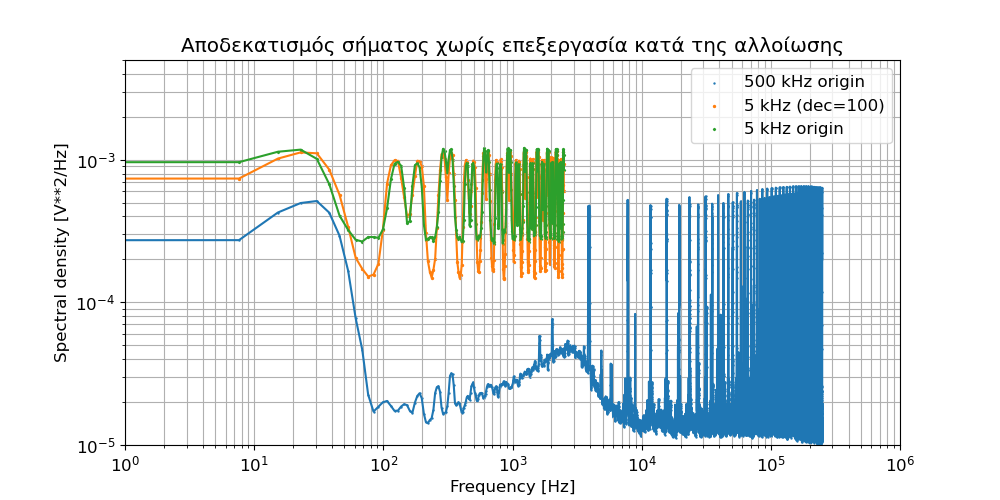
\includegraphics[width=500px,height=280px]{./decimation/with_aliasing.png}
\caption{Αποδεκατισμένο σήμα ανά 100 δείγματα (5 \en{kHz}) μαζί με το αρχικά καταγεγραμμένο σε μικρότερη συχνότητα 5 \en{kHz} σε σύγκριση με εκείνο στα 500 \en{kHz}.}
\end{figure}
\subsection{Μείωση αριθμού δειγμάτων}
\label{sec:orgb3fa50b}
Η τεχνική αυτή εφαρμόζεται σε ψηφιακά σήματα με πολλά δείγματα ανά
χρονικό διάστημα που όμως η τυπική απόκλιση προδίδει μια περιοδική
κίνηση που σχετίζεται με ταλάντωση. Τότε είναι εύλογο να χωριστεί το
σήμα σε μικρότερα “κομμάτια”. Αυτό έχει σαν αποτέλεσμα την ταχύτερη
ανάλυση των δεδομένων και την ευελιξία της επιλογής περιοχών του σήματος σε
συνάρτηση με τον χρόνο ή κάποιο άλλο κριτήριο. Εφαρμόζεται συχνά στην
καθημερινότητά μας, καθώς η συμπίεση αρχείων και τα πρότυπα αρχεία ήχου
και εικόνας συμπεριλαμβάνουν μία ή και περισσότερες διαδικασίες μείωσης
του αριθμού των δειγμάτων.

Στην επεξεργασία ψηφιακών σημάτων οι όροι μείωση αριθμού δειγμάτων,
αποδεκατισμός και συμπίεση μπορεί να έχουν ταυτόσημα νοήματα. Μπορεί όμως,
να περιγράφουν την απομείωση συχνοτήτων και απόρριψη αριθμού δειγμάτων σε
ένα σύστημα ψηφιακής καταγραφής σημάτων πολλαπλών συχνοτήτων. Αργότερα
θα αναλυθεί η σημασία τέτοιων συστημάτων.
\subsubsection{Ορισμός}
\label{sec:org050d90a}
Αποδεκατισμός ενός ψηφιακού σήματος σημαίνει η αποθήκευση τελικώς του
κάθε 10ου π.χ. δείγματος από το αρχικό καταγεγραμμένο σήμα με συγκεκριμένη
συχνότητα καταγραφής. Αυτό έχει επεκταθεί ορίζοντας τον αποδεκατισμό
κατά έναν παράγοντα που συνήθως είναι σταθερός αριθμός και μπορεί να
λάβει ακέραιες και δεκαδικές τιμές.

H ανάγκη να λαμβάνει ο παράγοντας αυτός μια λογική τιμή γίνεται αντιληπτή
από ένα απλό παράδειγμα. Για ένα ψηφιακό σήμα που έχει διάρκεια πέντε (5)
δευτερόλεπτα και καταγράφηκε από συσκευή που είχε συχνότητα καταγραφής 20
\en{Hertz}, ένας παράγοντας αποδεκατισμού 101, προφανώς δεν θα άφηνε κανένα
δείγμα στο νέο ψηφιακό σήμα. Επιπρόσθετα το όριο για να αποφύγουμε την
αλλοίωση απαιτεί το τελικό αποτέλεσμα των διαδικασιών να είναι τα 10 δείγματα ανά δευτερόλεπτο
(10 \en{Hz}). Επομένως θέτοντας τον παράγοντα αποδεκατισμού 51 θα παρείχε ένα
σήμα που θα ήταν αλλοιωμένο. Όταν η διαδικασία αυτή εφαρμόζεται σωστά σε
μια αλληλουχία δειγμάτων ενός σήματος ή μιας συνεχούς συνάρτησης, παράγεται
μια προσομοίωση του καταγεγραμμένου με μικρότερη συχνότητα.
\subsubsection{Ένα φίλτρο ως παράδειγμα}
\label{sec:org6361407}
Όταν το φίλτρο κατά της αλλοίωσης είναι σχεδιασμένο με πρότυπο \en{IIR}, τα
οποία θα αναλυθούν παρακάτω, η διαδικασία βασίζεται στην ανάδραση της
εξόδου στην είσοδο του φίλτρου πριν την έναρξη του δεύτερου σταδίου. Για
το πρότυπο σχεδιασμού \en{FIR} είναι εύκολο να υπολογιστεί για κάθε Μ εξόδου.
Ο υπολογισμός που γίνεται από ένα τέτοιο φίλτρο αποδεκατισμού για κάθε
νιοστή έξοδο δείγματος φαίνεται παρακάτω.

\begin{equation}
y[n]=\sum_{k=0}^{K-1}x[nM-k] \cdot h[k],
\end{equation}


Όπου η ακολουθία \en{h}[\(\cdot\)] είναι η απόκριση του κρουστικού παλμού (\en{impulse\ response})
, και K είναι το μήκος. Η \en{x}[\(\cdot\)] αντιπροσωπεύει το σήμα εισόδου
εξαγόμενο από το φίλτρο με λιγότερα δείγματα.
Σε επεξεργαστές γενικής χρήσης μετά τον υπολογισμό της παραπάνω εξίσωσης
για κάποιον αριθμό \en{n}, ο ευκολότερος τρόπος να υπολογιστεί το \en{y[n+1]}
είναι η καθυστέρηση της αρχής της ακολουθίας \en{x}[\(\cdot\)] κατά Μ, και να λυθεί
το παραπάνω άθροισμα ξανά. Αν ο παράγοντας Μ=2, η συνάρτηση \en{h}[\(\cdot\)] μπορεί
να αντιπροσωπεύει ένα φίλτρο μισών συχνοτήτων, όπου σχεδόν το μισό πλήθος
των δειγμάτων του αρχικού σήματος θα είναι μηδενικής ισχύος (\en{amplitude})
και δεν θα συμπεριληφθούν στο προϊόν πολλαπλασιασμού.
Οι \textbf{τιμές} της απόκρισης του παλμού κατά διαστήματα Μ δημιουργούν
υποαληλλουχίες, πλήθους Μ περιπλεγμένες μεταξύ τους.Το παράγωγο του
πολλαπλασιασμού είναι η πρόσθεση των προϊόντων από τον πολλαπλασιασμό
κάθε υποαληλλουχίας με το καταγεγραμμένο σήμα \en{x}[\(\cdot\)]. Επιπρόσθετα λόγω
της μείωσης του πλήθους των δειγμάτων στο σήμα κατά Μ, κάθε σήμα που
χρησιμοποιήθηκε στον προηγούμενο υπολογισμό κάποιου Μ προϊόντος δεν θα
επαναληφθεί σε επόμενο υπολογισμό. Αυτός είναι και ο λόγος που τα φίλτρα
μικρής τάξης Μ \en{FIR} φιλτράρουν μια από τις αλληλουχίες της εισόδου κάθε
φορά και τα Μ προϊόντα προσθέτονται για να κατασκευαστεί το σήμα εξόδου.
Αυτή η μέθοδος εφαρμόζεται σε συστήματα πολλαπλών επεξεργαστών, όπου ένα
σήμα χωρίζεται σε φάσεις και φιλτράρεται ξεχωριστά από Μ αριθμό φίλτρων
και τελικά προσθέτονται για την δημιουργία του σήματος εξόδου. Τα παραπάνω
φίλτρα ονομάζονται και πολυφασικά.

Για εγκυκλοπαιδικούς λόγους αξίζει να σημειωθεί πως είναι πιθανό σε κάθε
φάση του υπολογισμού να αντικαθιστούμε τις τιμές της προηγούμενης φάσης
με μηδενικές τιμές, σε ένα αντίγραφο της αλληλουχίας \en{h}[\(\cdot\)], ώστε να
επεξεργαστεί το αρχικό σήμα στην συχνότητα εισόδου (πολλαπλασιάζοντας
με 0) και αποδεκατίζοντας την έξοδο κατά έναν παράγοντα Μ. Η παραπάνω
διαδικασία ονομάστηκε στα αγγλικά \en{the\ first\ Noble\ identity} και εφαρμόζεται σε
διάφορες πολυφασικές μεθόδους.
\subsection{Κατηγορίες Φίλτρων}
\label{sec:org88a3e8b}
Λόγω των πολλών εφαρμογών που έχουν και την εκθετική αύξηση της χρήσης
ηλεκτρονικών συσκευών στην καθημερινότητα, οι δυνατότητες επεξεργασίας
ψηφιακών σημάτων αποτελεί πρακτικά απαραίτητη προϋπόθεση. Έτσι η ανάγκη
για την ανάπτυξη διαφόρων τύπων φίλτρων, π.χ. το φίλτρο μέσης τρέχουσας
τιμής (\en{F.I.R.}), το φίλτρο άπειρης κρουστικής απόκρισης (\en{I.I.R.}) και το μεσιανό
φίλτρο \en{median\ filters}, έγινε εμφανής από το στάδιο ακόμα της ανάπτυξης
του ραδιοφώνου. Στην συνέχεια θα αναφερθούμε στις δύο από τις τρεις αυτές
κατηγορίες αναφέροντας παραδείγματα από τις μεθόδους που χρησιμοποιήθηκαν
στην ανάλυση των δεδομένων από την εργαστηριακή εγκατάσταση.
Η γενική διαφοροποίηση που γίνεται αρχικά είναι ως προς το εύρος
συχνοτήτων που επηρεάζουν. Έτσι αν απορρίπτονται οι υψηλές συχνότητες, το
φίλτρο ονομάζεται διέλευσης χαμηλών συχνοτήτων (\en{low-pass\ filter})
ενώ το αντίστροφο ονομάζεται φίλτρο διέλευσης υψηλών συχνοτήτων (\en{high-pass\ filter}).
Αν το φίλτρο επηρεάζει μία περιοχή ή \textbf{φάσμα} συχνοτήτων και
απορρίπτει όσες βρίσκονται πριν και μετά, ονομάζεται φίλτρο διέλευσης
εύρους συχνοτήτων (\en{band-pass\ filter}).
\subsubsection{Φίλτρα διέλευσης και απόρριψης συχνοτήτων}
\label{sec:org521d12b}
Τα φίλτρα διέλευσης ορίζονται ως εκείνα που επιτρέπουν την διατήρηση του
εύρους συχνοτήτων που βρίσκονται στην ουδέτερη περιοχή του φίλτρου από την είσοδο στην
έξοδο. Για τα φίλτρα χαμηλών συχνοτήτων το εύρος είναι από την συχνότητα
κατακρημνισμού και πριν, ενώ για εκείνα των υψηλών το αντίθετο (μέχρι την
μέγιστη καταγεγραμμένη συχνότητα). Στην πράξη χρησιμοποιούμε τα φίλτρα
διέλευσης όταν δεν γνωρίζουμε το εύρος του σήματος που επηρεάζεται
από τον θόρυβο, αλλά μπορούμε να περιορίσουμε μια περιοχή μέχρι
κάποια γνωστή συχνότητα που επιθυμούμε να συμπεριλάβουμε στο σήμα εξόδου.

Φίλτρο απόρριψης συχνοτήτων χρησιμοποιείται συνήθως όταν γνωρίζουμε το εύρος
που επιθυμούμε να αφαιρέσουμε από το επεξεργασμένο σήμα. Ενώ για τα φίλτρα
διέλευσης μπορούν να χρησιμοποιηθούν εκείνα των χαμηλών, υψηλών αλλά και
εύρους συχνοτήτων στην δεύτερη υποκατηγορία, νόημα έχουν μόνο για τα φίλτρα
εύρους συχνοτήτων.
Αυτό συμβαίνει καθώς ένα φίλτρο απόρριψης χαμηλών συχνοτήτων είναι ουσιαστικά
διέλευσης υψηλών συχνοτήτων. Λόγω της προαναφερόμενης επικάλυψης, χρησιμοποιούμε
φίλτρα απόρριψης όταν είναι ξεκάθαρο ένα ενδιάμεσο εύρος συχνοτήτων που κρίνεται
ως θόρυβος, αλλά οφείλουμε να διατηρήσουμε όλο το εύρος πριν και μετά από αυτό.
\subsection{Φίλτρο μέσης τρέχουσας τιμής}
\label{sec:org26da7b7}
Στα προηγούμενα κεφάλαια επικεντρωθήκαμε περισσότερο στην μαθηματική αναπαράσταση
των σημάτων, με μια μικρή αναφορά στα γραμμικά συστήματα. Τα φίλτρα αποτελούν γραμμικά
συστήματα και ως εκ τούτου αντιμετωπίζονται, λαμβάνοντας υπόψη τις ανάλογες ιδιότητες
και συμπεριφορές. Σκοπός σχεδιασμού αυτών των συστημάτων αποτελεί η αφαίρεση στοιχείων
από κάποιο σήμα, ή η τροποποίηση προκαθορισμένων χαρακτηριστικών του. Εδώ θα αναφερθούμε
στην κατηγορία των συστημάτων πεπερασμένης κρουστικής απόκρισης, ή όπως θα αποκαλούνται
στην συνέχεια για συντομία \en{F.I.R.}. Για αρχή μπορούμε να φανταστούμε πως η έξοδος του
φίλτρου παράγεται αθροίζοντας ένα πεπερασμένο αριθμό δειγμάτων όπου εφαρμόζουμε κάποιο
“βάρος στάθμισης”. Στόχος των επόμενων ενοτήτων είναι ο προσδιορισμός των βασικών αρχών,
πού διέπουν τα διακριτά συστήματα και την εφαρμογή τους στον σχεδιασμό των \en{F.I.R.}. Θα
επανέλθουμε στον όρο της γραμμικότητας και θα αναφερθούμε και στην χρονική αμεταβλητότητα
που συνδυασμένες καλύπτουν ένα ευρύ φάσμα της εν' λόγω κατηγορίας.
\subsubsection{Μέση τρέχουσα τιμή και σχεδιασμός συστήματος}
\label{sec:org7a2ec1b}
Ένας από τους πιο διαδεδομένους τρόπους μετασχηματισμού σημάτων είναι ο υπολογισμός
της μέσης τιμής για δύο ή παραπάνω δείγματα, με σκοπό την αφαίρεση έντονων στιγμιαίων
διακυμάνσεων του σήματος γύρω από κάποια επιθυμητή τιμή. Λόγω της πληθώρας αλγόριθμων
για τον υπολογισμό μέσης τιμής ακολουθιών, είναι από τις πιο συχνά εφαρμοσμένες τεχνικές
στον τομέα της οικονομικής επιστήμης. Πιο συγκεκριμένα, στην μακροχρόνια ανάλυση των
τιμών μετοχής σε χρηματιστήριο, εφαρμόζεται για τον υπολογισμό της μετοχής, σε συνάρτηση
της απόκλισης λόγω οικονομικών φαινομένων. Με απλά λόγια, αν κάποιος επιθυμεί να εξετάσει
την ανοδική ή καθοδική πορεία μιας μετοχής δεν τον αφορά η αυξομείωση της τιμής ανά ημέρα,
πόσο μάλλον ανά δευτερόλεπτο. Τα τελευταία δεκαδικά όμως αλλάζουν κάθε δευτερόλεπτο, σε
πραγματικό χρόνο και επομένως εφαρμόζεται ένα φίλτρο μέσης τρέχουσας τιμής,
ώστε να είναι δυνατή η αξιοποίηση της πληροφορίας των μεταβολών, με μικρότερη απόκλιση,
από την μέση τιμή.

Για να γίνει πιο κατανοητό ας υποθέσουμε πως ένα ψηφιακό σήμα μπορεί να αναπαρασταθεί
ως \en{in[z]}. Εφαρμόζεται ένα σύστημα φίλτρου όπως του ανωτέρω παραδείγματος, υπολογίζοντας
τον μέσο όρο από πέντε δείγματα την φορά. Τότε για κάθε δείγμα της ακολουθίας εξόδου του
συστήματος θα ισχύει ότι:
\begin{align}
\label{fir~filter}
out[n] = \frac{1}{k} \cdot \sum_{z}^{{k-1}}in[n+z], k=5
\end{align}
Η ανωτέρω σχέση \ref{fir~filter} ονομάζεται και σχέση διαφορών, αποτελώντας πλήρη περιγραφή ενός \textbf{συστήματος \en{F.I.R}}, δίνοντας την δυνατότητα στον χρήστη να εξάγει πληροφορία για κάθε τιμή του σήματος
εισόδου \en{in[n]}. Όσο για τον προσδιορισμό της αρχικής τιμής της μεταβλητής \en{z}, τις περισσότερες
φορές επιλέγεται η τιμή μηδέν με σκοπό να συμπεριλάβουμε το πρώτο δείγμα της εισόδου,
στο οποίο αναφερόμαστε εδώ και στην συνέχεια ως \en{in[0]}. Το δείγμα που λαμβάνεται σαν “αρχικό”,
για \en{n = [1,\ 2,\ 3,\ \(\ldots\)] } μπορούμε να το χαρακτηρίσουμε και ως το παρόν του σήματος. Αντίστοιχα τα
δείγματα που έπονται αυτού, και χρησιμοποιούνται στο παραπάνω σύστημα για τον υπολογισμό
της εξόδου, συνθηκολογώντας αναφέρονται στην βιβλιογραφία ως μέλλον του σήματος.

\begin{figure}[H]
\centering
\includegraphics[height=220px]{./.ob-jupyter/14cddadf93f57c680a0d2666349763fb2ab40d27.png}
\caption{\label{fig_explaining_future}Παράδειγμα απεικόνισης παραθύρου και της έννοιας του παρελθόντος και μέλλοντος σήματος.}
\end{figure}

Η συγκεκριμένη οπτική εντάσσει την έννοια των “παραθύρων” καθώς ένα συρόμενο παράθυρο, πέντε
τιμών συνεχίζοντας το παράδειγμα, θα ορίσει τις επιλεγμένες τιμές για τον υπολογισμό του
σήματος εξόδου \en{out[n]}.
\subsubsection{Σχεδιασμός και εφαρμογή φίλτρων}
\label{sec:orgc2d7dcc}
Ένα \en{F.I.R.} φίλτρο κατασκευάζεται από την γενική εξίσωση διαφορών που θα δούμε παρακάτω,
όμως αξίζει να αναφέρουμε ένα χαρακτηριστικό. Για τα φίλτρα που κατασκευάζονται
χρησιμοποιώντας στοιχεία του παρελθόντος από το σήμα εισόδου για τον υπολογισμό της μέσης τιμής,
έχει επικρατήσει η ονομασία αιτιατό φίλτρο. Με την συγκεκριμένη έκφραση εννοούμε πως
η αιτία που καθορίζει το αποτέλεσμα δεν προηγείται αυτού. Αντίστοιχα τα φίλτρα που
βασίζονται σε στοιχεία που προπορεύονται του εξεταζόμενου στοιχείου ονομάζονται μη
αιτιατά. Ας δούμε την γενική εξίσωση που καθορίζει ένα φίλτρο όπως ορίστηκε παραπάνω,
για κάποιο αιτιατό φίλτρο μέσης τρέχουσας τιμής.
\begin{align}
out[x] = \sum_{z=0}^{{T}} a_{z} in[x-z]
\end{align}

Γίνεται λοιπόν αντιληπτό πως, λόγω του πεπερασμένου πεδίου ορισμού του σήματος εισόδου
και της διακριτότητας του φάσματός του, θα υπάρχουν στοιχεία κατά τον υπολογισμό των
αρχικών δειγμάτων εξόδου σε ένα παράθυρο αντίστοιχο εκείνο του αριθμού Τ, που βασίζονται
σε λιγότερα από πέντε στοιχεία. Αυτό στις εφαρμογές των φίλτρων προβλέπεται και κατ'
επέκταση δίνεται η δυνατότητα ο δείκτης \en{z} να λάβει αρνητικές τιμές. Στην αρχή μοιάζει
παράδοξο, καθώς δεν μπορεί στην φύση να υπάρξει αρνητικός αριθμός δειγμάτων, όμως μας
δίνει την δυνατότητα να εφαρμόζουμε σχετικά μεγάλα παράθυρα, χωρίς τον φόβο διαστρέβλωσης
της εξόδου.

Ένα φίλτρο για να οριστεί πλήρως, είναι απαραίτητο να γνωρίζουμε με σαφήνεια όλες τις
τιμές των συντελεστών του, δηλαδή των \en\{a\textsubscript{z}\} στο παράδειγμα που παρουσιάστηκε το αιτιατό φίλτρο.
Υποθέτοντας τις παρακάτω τιμές για το σύνολο αυτό, μπορούμε να γνωρίζουμε την εξίσωση
που περιγράφει το ανάλογο φίλτρο π.χ.:
\begin{align}
\nonumber
\{a_{z}\} = \{5,\ -7,\ 2,\ 1,\ 9\} \Rightarrow\\
out[x] &= \sum_{z=0}^{4}a_{z}in[x-z]\\
\nonumber
&= 5in[x] - 7in[x-1] + 2in[x-2] + in[x-3] +9in[x-4]
\end{align}

Όπως φαίνεται είμαστε σε θέση να υπολογίσουμε το σήμα εξόδου για κάθε τιμή της εισόδου.
Ο αριθμός Τ ονομάζεται τάξη του φίλτρου ενώ το πλήθος των συντελεστών ονομάζεται μήκος ή
μέγεθος. Οι έννοιες αυτές προέρχονται από τον μετασχηματισμό \en{Z}, μέθοδος η οποία  ξεπερνά
το πλαίσιο της παρούσας εργασίας. Ας συνδέσουμε για λόγους κατανόησης, το μήκος με την
ταχύτητα υπολογισμού του φίλτρου, ενώ την τάξη με την μεταβολή της ταχύτητας κατακρημνισμού της
εξίσωσης του φίλτρου ή όπως ονομάζεται στα περισσότερα όργανα ηλεκτρονικής μουσικής
\en{release\ value}.
\subsection{Φίλτρο άπειρης κρουστικής απόκρισης}
\label{sec:orga5982d4}
Τα φίλτρα άπειρης κρουστικής απόκρισης είναι, όπως προδίδει και το όνομά τους,
ακριβώς το αντίθετο από εκείνα της πεπερασμένης. Πρακτικά αυτό σημαίνει
πως η διάρκεια της κρουστικής απόκρισης είναι άπειρη. Συμπερασματικά, καθώς ο
υπολογισμός γίνεται χρησιμοποιώντας την μέθοδο της ανάδρασης, αξιοποιούμε την
έξοδο του φίλτρου για την επανατροφοδότηση της εισόδου. Η γενική εξίσωση της
παρούσας κατηγορίας έχει την μορφή:
\begin{align}
out[z] = \sum_{f=0}^{\infty}u(f)in(z-f)
\end{align}

Όπως είναι φανερό η διαφορά εδώ είναι πως το άνω όριο της πρόσθεσης προσεγγίζει
το άπειρο, σε θεωρητικό επίπεδο τουλάχιστον. Αυτό συμβαίνει γιατί η απόκριση
της ακολουθίας \en{u} διαθέτει άπειρη διάρκεια. Έτσι όπως θα δειχθεί αμέσως μετά,
ο υπολογισμός με την μέθοδο της συνέλιξης καθίσταται μη πρακτικός και εφαρμόζεται
αναδρομή. Για να γίνει πιο κατανοητή η έννοια της αναδρομής ας δούμε ένα
παράδειγμα που, κατά την σωστή εφαρμογή του, απαιτούνται I+T+1
πολλαπλασιασμοί και I+T αθροίσεις για τον υπολογισμό της απόκρισης του φίλτρου.
\begin{align}
out[z] = - \sum_{f=1}^{T}c(f)out(z-f) + \sum_{f=0}^{I}d(f)in(z-f)
\end{align}

Σημαντικό μειονέκτημα των \en{IIR} φίλτρων είναι η διαφορά φάσης που παράγεται στην
έξοδό τους. Αν είναι ζωτικής σημασίας, τότε υπερτερούν τα \en{FIR}, αφού ο υπολογισμός
της απόκρισης των συστημάτων απειροστού μεγέθους απαιτεί μη γραμμική ανάλυση.
Στην αντίθετη περίπτωση η τάξη (\en{order}) του φίλτρου, για την απόρριψη του ίδιου
φάσματος συχνοτήτων ενός σήματος θα είναι πολύ μικρότερη κάνοντας χρήση της
αναδρομικής ιδιότητας των \en{IIR}. Στην επόμενη ενότητα φαίνονται κάποια παραδείγματα
με τον αντίστοιχο κώδικα σε \en{python} για την δημιουργία δειγμάτων των βασικών
αποκρίσεων σε συνάρτηση του αριθμού δειγμάτων. Αρχικά φαίνονται έντονες
διαφορές στην απόκριση που παρέχουν όμως όλα υπολογίζονται με την χρήση των
παραπάνω εξισώσεων. Εξαίρεση απαιτεί το φίλτρο \en{butterworth} που
λεπτομέρειες θα αναφέρουμε στην συνέχεια.
\clearpage
\subsubsection{Παραδείγματα με κώδικα}
\label{sec:orge7532d5}
\selectlanguage{greek}
Εδώ φαίνονται μερικά από τα βασικότερα φίλτρα άπειρης κρουστικής απόκρισης, που
από εδώ και πέρα θα αναφερόμαστε σε αυτά ως \en{IIR}. Οι τύποι των παρακάτω φίλτρων
αποτελούν τα πιο διαδεδομένα και εύχρηστα, για την προσομοίωση φυσικών εφαρμογών
σε προγραμματιστικό περιβάλλον. Δεν είναι άλλωστε τυχαίο πως οι περισσότερες
γλώσσες προγραμματισμού παρέχουν μια ή και περισσότερες βιβλιοθήκες για τον
σχεδιασμό και τη χρήση τους.

Το φίλτρο \en{butterworth} αποτελεί την καλύτερη δυνατή λύση για έξοδο με την μικρότερη
ενίσχυση καθώς όπως φαίνεται και στο γράφημα δεν παρουσιάζει ταλαντωτικές
συμπεριφορές στις συχνότητες διέλευσης και απόρριψης. Αυτό επιτυγχάνεται
μειώνοντας την ταχύτητα μεταβολής της ισχύος του σήματος, αποκτώντας έτσι μια
περιοχή μετάβασης όπου οι συχνότητες δεν απορρίπτονται όμως απομειώνονται σε
σημαντικό βαθμό ώστε να μην αλλοιώνεται η έξοδος του.

Παρακάτω φαίνεται η κατασκευή ενός πρότυπου φίλτρου τύπου \en{butterworth} με την χρήση
της βιβλιοθήκης \en{scipy}. Αντίστοιχα παραδείγματα θα προστεθούν για κάθε γράφημα
πρότυπου φίλτρου.

\selectlanguage{english}
\begin{minted}[]{python}
from scipy import signal
import matplotlib.pyplot as plt
import numpy as np

bb, ab  = signal.butter (4, 100, 'low', analog=True, output='ba')
wb, hb = signal.freqs(bb, ab)
\end{minted}

\selectlanguage{greek}
\begin{figure}[htbp]
\centering
\includegraphics[height=200px]{./Butterworth Filter Freq Response.png}
\caption{Πρότυπο φίλτρο τύπου \en{Butterworth} τέταρτης τάξης με συχνότητα κατακρημνισμού εκατό \en{Hz}.}
\end{figure}

Ο λόγος που αναφερόμαστε στην ισχύ σε ντεσιμπέλ, προκύπτει από την ανάγκη
να εντοπίσουμε μεταβολές μικρής κλίμακας στην ισχύ που αντιπροσωπεύουν
ισχυρές μεταβολές στο σύστημα που καταγράφουν.

Στα διαγράμματα εδώ παρουσιάζονται διαφορετικού τύπου φίλτρα διέλευσης
χαμηλών συχνοτήτων, με συχνότητα κατακρημνισμού \en{100\ Hz}. Ο οριζόντιος άξονας
εκφράζει την συχνότητα καταγραφής, ενώ ο κάθετος απεικονίζει την ισχύ του
σήματος στην αντίστοιχη συχνότητα. Η ισχύς εκφράζεται σε \en{decibel\ [dB]} μονάδα
που ορίζεται ως λόγος ισχύων, αφού γνωρίζουμε την ισχύ του σήματος που
καταγράψαμε. Σε άλλες περιπτώσεις θα μπορούσαμε να εκφράσουμε λόγο εντάσεων
σε ντεσιμπέλ επίσης. Υπολογίζεται ως το δεκαπλάσιο του λογαρίθμου του
εκάστοτε λόγου, για παράδειγμα:

\begin{align}
A_{dB} = 10 \cdot \log10\left[{\frac{I_{1}}{I_{0}}}\right]
\end{align}

\selectlanguage{english}
\begin{minted}[]{python}
bb, ab = signal.bessel (4, 100, 'low', analog=True, output='ba')
wb, hb = signal.freqs(bb, ab)
\end{minted}
\selectlanguage{greek}
\begin{figure}[htbp]
\centering
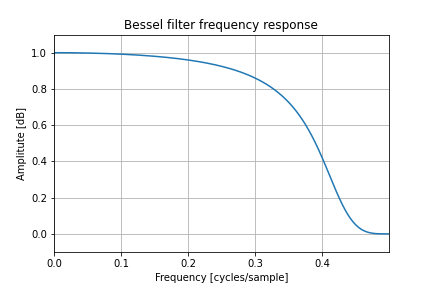
\includegraphics[height=200px]{./Bessel Filter Freq Response.png}
\caption{Πρότυπο φίλτρο τύπου \en{Bessel} τέταρτης τάξης με συχνότητα κατακρημνισμού εκατό \en{Hz}.}
\end{figure}

Στην εγκατάσταση καταγράφηκε μεταβολή στην ισχύ του σήματος από 1.62 μονάδες
για ταχύτητα \en{0\ m/s} σε 1.76 για ταχύτητα \en{10\ m/s} για το πείραμα του
πεπιεσμένου αέρα. Στην περίπτωση της αεροσήραγγας η διαφορά κυμαίνεται από
1.623 σε 2.05 αντίστοιχα. Η λογαριθμική κλίμακα προσφέρει καλύτερη απεικόνιση
και εστίαση στο εύρος συχνοτήτων που περιέχουν την πληροφορία της ταχύτητας
του ανέμου (εδώ ήταν οι χαμηλές συχνότητες).

Το \en{chebyshev} ενώ εκ πρώτης όψης φαίνεται να επηρεάζει το σήμα σε μη
αποδεκτό βαθμό, προνόμιό του αποτελεί η ταχύτητα που προσφέρει αποτελέσματα.
Αυτό οφείλεται στην μέθοδο της αναδρομής που χρησιμοποιείται κατά την επεξεργασία
με το συγκεκριμένο φίλτρο. Τα περισσότερα χρησιμοποιούν την μέθοδο της συνέλιξης.
Το \en{elliptic} παρουσιάζει εξαιρετική ταχύτητα επεξεργασίας με αδυναμία στην
ποιότητα της εξόδου λόγω των κυματισμών.

\clearpage
\selectlanguage{english}
\begin{minted}[]{python}
bb, ab = signal.cheby1 (4, 2, 100, 'low', analog=True, output='ba')
wb, hb = signal.freqs(bb, ab)
\end{minted}
\selectlanguage{greek}
\begin{figure}[htbp]
\centering
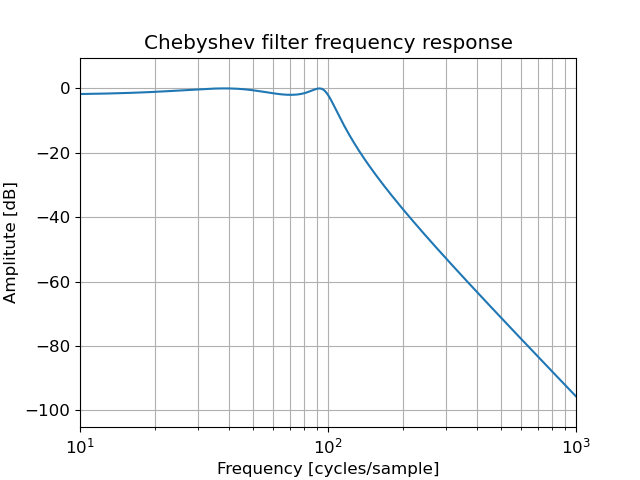
\includegraphics[height=210px]{./Chebyshev Filter Freq Response.png}
\caption{Πρότυπο φίλτρο τύπου \en{Chebyshev} τέταρτης τάξης με συχνότητα κατακρημνισμού εκατό \en{Hz} και αριθμό κυματισμών ίσο με δύο.}
\end{figure}

\selectlanguage{english}
\begin{minted}[]{python}
bb, ab = signal.ellip (4, 2, 8, 100, 'low', analog=True, output='ba')
wb, hb = signal.freqs(bb, ab)
\end{minted}
\selectlanguage{greek}
\begin{figure}[htbp]
\centering
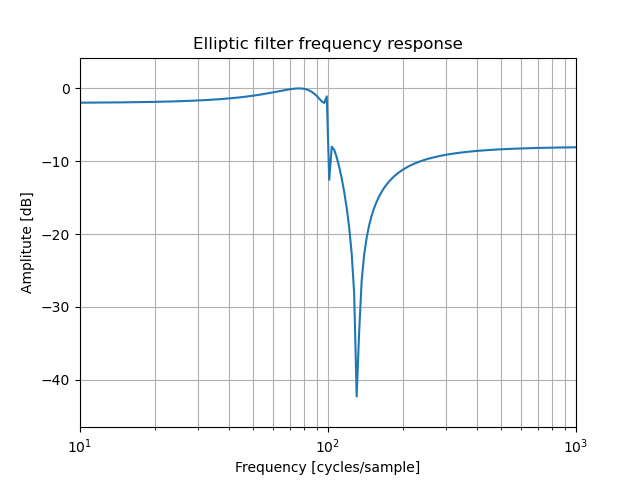
\includegraphics[height=210px]{./Elliptic Filter Freq Response.png}
\caption{\label{ellipt}\en{Elliptic} τέταρτης τάξης με συχνότητα κατακρημνισμού εκατό \en{Hz} και μέγιστη αύξηση ισχύος κατά 2 \en{dB} στην περιοχή διέλευσης (κυματισμοί) ενώ οκτώ \en{dB} ελάχιστα στην περιοχή απομείωσης.}
\end{figure}

\vfill
\section{Μεθοδολογία}
\label{sec:org78e8986}
\subsection{Εγκατάσταση εργαστηρίου}
\label{sec:orge495cd8}
    Η εγκατάσταση που χρησιμοποιήθηκε για την συλλογή των δεδομένων
αποτελείται από μία αεροσήραγγα την οποία τροφοδοτεί με σταθερή ταχύτητα
αέρα, ηλεκτροκινητήρας προσδεδεμένος σε έναν έλικα. Στην μέση της
σήραγγας υπάρχει ένα πλέγμα διάχυσης ώστε η ροή του αέρα να γίνεται όσο
το δυνατόν πιο ομοιόμορφα στην έξοδο όπου βρίσκεται και το αισθητήριο
όργανο για την καταγραφή της ταχύτητας του ανέμου.

\begin{figure}[htbp]
\centering
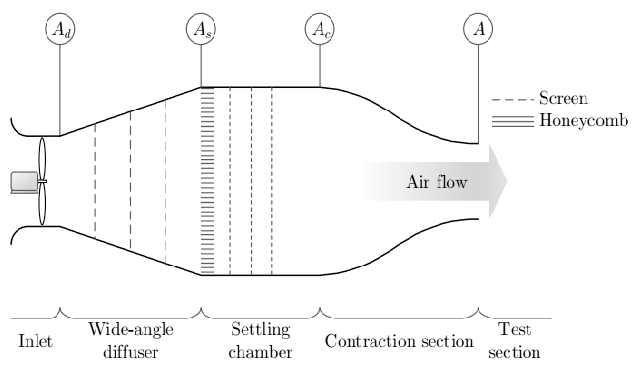
\includegraphics[width=420px,height=250px]{./Wind_Tunnel_setup_lab.png}
\caption{Θάλαμος ομοιόμορφης παροχής ανέμου στο αισθητήριο όργανο όπου τοποθετείται στο σημείο \textbf{Α}. Στο σημείο  \textbf{\(A_{s}\)}, βρίσκεται ένα πλέγμα διάσπασης της ροής που μας επιτρέπει την ομαλή ταχύτητα στο σημείο εξόδου \textbf{A}.}
\end{figure}

Στο παραπάνω σκίτσο απεικονίζεται η μορφολογία της αεροσήραγγας ώστε να
επιτευχθεί ομαλή ροή ανέμου προς το αισθητήριο όργανο. Στη συνέχεια γίνεται
καταγραφή του αισθητήρα με ειδική κάρτα επεξεργασίας σημάτων της εταιρίας
\en{National\ Instruments } μοντέλο \en{USB-6353}. Περισσότερα για τον τρόπο σύνδεσης και
την μέθοδο καταγραφής θα παρατεθούν αμέσως μετά. Αξίζει όμως να σημειωθεί
πως η κατασκεύη έγινε στην Κρήτη με την συμβολή ξυλουργού που ενήργησε με την
καθοδήγηση σχεδίων από προσωπικό της σχολής.
\subsection{Μεθοδολογία καταγραφής}
\label{sec:org419a60a}
Για την σύνδεση της κάρτας επεξεργασίας χρησιμοποιήθηκε σειριακή θύρα \en{USB} και
για την καταγραφή το λογισμικό \en{Lab\ View}, όπου αποθήκευσε τα δεδομένα σε μορφή
\en{.tdms}. Για την αποκωδικοποίηση των αρχείων υπάρχουν βιβλιοθήκες σχεδόν για όλες
τις γλώσσες προγραμματισμού. Στο διάγραμμα ροής εμφανίζεται μια διακεκομμένη
γραμμή. Έτσι υποδεικνύεται πως δεν υφίσταται επεξεργασία το σήμα κατά την
καταγραφή. Η επιλογή της συχνότητας καταγραφής γίνεται στο λογισμικό και μας
προσφέρει την δυνατότητα για έως και \en{500\ kHz}.
\begin{figure}[htbp]
\centering
\includegraphics[width=.9\linewidth]{./flowcharts/recording.png}
\caption{Διάγραμμα ροής για την μέθοδο καταγραφής και τις περιπτώσεις που εξετάστηκαν.}
\end{figure}
\subsection{Μεθοδολογία επεξεργασίας}
\label{sec:org11fdbd6}
Ένας λόγος που δεν χρησιμοποιήθηκε επεξεργασία σε πραγματικό χρόνο είναι
ότι η εγκατάσταση που χρησιμοποιήθηκε για την συλλογή των δεδομένων,
κατασκευάστηκε με σκοπό την σύνδεσή του σε κεντρική μονάδα επικοινωνίας,
και έπειτα, πραγματοποιείται σύνδεση μέσω σειριακής θύρας \en{USB} με Η/Υ,
όπου και καταγράφεται το σήμα του αισθητήριου οργάνου (\en{pitot-tube}). Ένας
δεύτερος λόγος, ήταν η ανάγκη να δοκιμαστούν διαφορετικές μέθοδοι
αφαίρεσης του θορύβου και προφανώς αυτό θα ήταν πιο δύσκολο εάν έπρεπε
να γίνει σε πραγματικό χρόνο αλλάζοντας τις απαραίτητες παραμέτρους για
την ρύθμιση του φίλτρου. Θα έπρεπε λοιπόν να εγκατασταθεί ανάλογη
συσκευή, όπως ένας μικροεπεξεργαστής, που θα είχε την δυνατότητα για
υψηλές ταχύτητες δειγματοληψίας καθώς η καταγραφή έγινε στα 100 και 500 \en{kHz}.
Αυτό θα αύξανε πολύ το κόστος της κατασκευής και θα απαιτούσε
βαθμονόμιση του φίλτρου, για να μην προστεθεί περαιτέρω σφάλμα στην
μέτρηση. Παρακάτω φαίνεται ένα διάγραμμα της συνδεσμολογίας και του τρόπου
καταγραφής του σήματος.
\begin{figure}[htbp]
\centering
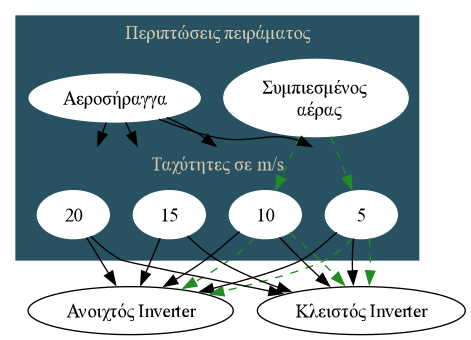
\includegraphics[height=252px]{./flowcharts/test-first.png}
\caption{\label{big_graph}Διάγραμμα ροής για την μέθοδο καταγραφής και τις περιπτώσεις που εξετάστηκαν.}
\end{figure}

Για την επεξεργασία των δεδομένων έπρεπε αρχικά να σιγουρευτούμε πως οι
μετρήσεις δεν υπέφεραν από το φαινόμενο της αλλοίωσης. Έτσι καθίσταται
αναγκαία η εφαρμογή της μεθόδου μείωσης αριθμού δειγμάτων, ώστε να εξεταστεί
το μέγεθος αλλοίωσης του σήματος. Στην συνέχεια έπρεπε να γίνει η μετατροπή
του σήματος στο πεδίο των συχνοτήτων για να αναγνωριστεί το φάσμα συχνοτήτων
που εμπεριέχει τον θόρυβο και να σχεδιαστεί το κατάλληλο φίλτρο. Για τον σκοπό
αυτό εφαρμόστηκε ο ταχύς μετασχηματισμός \en{Fourier} από την βιβλιοθήκη \en{numpy} και
φάνηκε ξεκάθαρα μια περιοχή συχνοτήτων στα σήματα από τα 2000 \en{Hz}, επηρεασμένα
από θόρυβο. Εδώ φαίνονται δύο από τα διαγράμματα της ανάλυσης των φίλτρων, που
χρησιμοποιήθηκαν στην σύγκριση των μεθόδων απόρριψης του θορύβου.

\begin{figure}
\centering
\begin{subfigure}{.5\textwidth}
\centering
\includegraphics[width=1. \linewidth]{./fir-filter-2000.png}
\caption{\en{F.I.R.} φίλτρο}
\label{fig:sub1}
\end{subfigure}%
\begin{subfigure}{.5\textwidth}
\centering
\includegraphics[width=1. \linewidth]{./iir-butter-2000.png}
\caption{\en{I.I.R.} φίλτρο}
\label{fig:sub2}
\end{subfigure}
\caption{Διαφορετικά φίλτρα διέλευσης χαμηλών συχνοτήτων}
\label{fig:test}
\end{figure}

Η εύρεση της μέσης τιμής για κάθε στοιχείο του σήματος με την συνάρτηση
\en{average()} για την ανάλυση του σήματος στο πεδίο του
χρόνου. Μας δίνει την πληροφορία της ισχύος του σήματος γύρω από την ενδιάμεση
τιμή, ή αλλιώς \textbf{θέση ισορροπίας ταλάντωσης}. Επιπρόσθετα η μέθοδος που
εφαρμόζεται για την εξέταση των φίλτρων και των άλλων διεργασιών που
εφαρμόζονται στο σήμα βασίζεται στην τεχνική του \en{Welch} για την εκτίμηση της
πυκνότητας φάσματος συχνοτήτων.

Έτσι για την εκλογή των συμπερασμάτων, θα παρατεθούν στη συνέχεια διαγράμματα
με το αρχικό σήμα και το επεξεργασμένο στο πεδίο των συχνοτήτων, αφού καθίσταται
ευκολότερο να διακρίνουμε την επιρροή των φίλτρων στο σήμα εξόδου. Όπως έχει
αναφερθεί και παραπάνω, κατά την απόρριψη του μή αποδεκτού θορύβου, τα φίλτρα
εντάσσουν καταστρεπτικές συμπεριφορές στο σύστημα που αν δεν ληφθούν
υπ' όψη ενδέχεται να επηρεάσουν το σήμα εξόδου.

\begin{figure}[htbp]
\centering
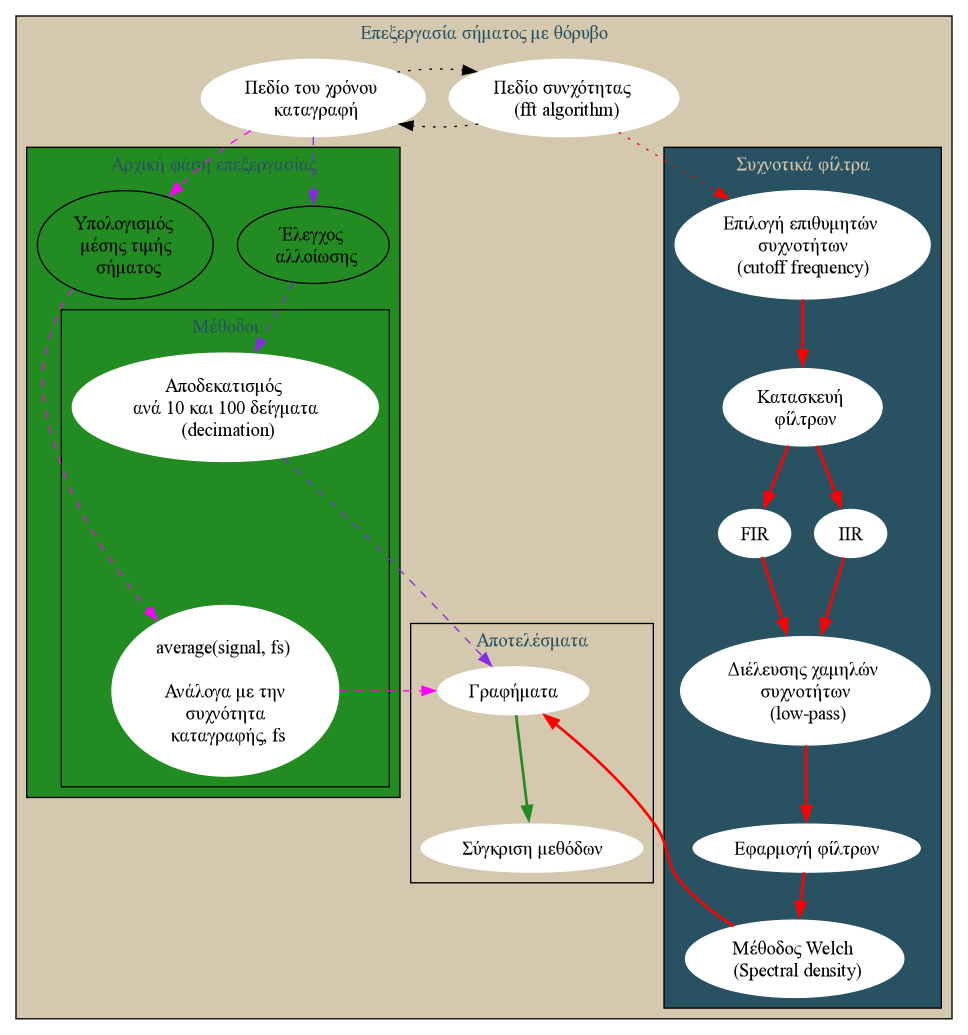
\includegraphics[width=.9\linewidth]{./flowcharts/proc-meth.png}
\caption{\label{more_in_depth}Μέθοδος ανάλυσης και επεξεργασίας σημάτων για την εκλογή καταλληλότερου φίλτρου διέλευσης χαμηλών συχνοτήτων.}
\end{figure}
\subsection{Μεθοδολογία σύγκρισης}
\label{sec:org25d6d08}
Για να συγκρίνουμε τις δυο διαφορετικές διαδικασίες είναι προφανές ότι δεν
ωφελεί να επικεντρωθούμε στην ταχύτητα έκδοσης αποτελεσμάτων. Θα πρέπει λοιπόν
να εξετάσουμε τις διαστρεβλώσεις σε χαμηλές συχνότητες που εντάσσει η κάθε
κατηγορία, αλλά και τη διαφορά φάσης της εξόδου κάθε διαδικασίας. Εύλογα έχουν
γίνει προσπάθειες για την εξάλειψη της καθυστέρησης που προκύπτει και οι
περισσότερες βιβλιοθήκες με σκοπό την επεξεργασία σημάτων, έχουν λύσει σε
τέτοιο βαθμό το πρόβλημα που σχεδόν δεν απασχολεί τον ερευνητή πέρα από την
επιλογή της κατάλληλης συνάρτησης. Για την επεξεργασία των δεδομένων έχουν ληφθεί
δύο μέτρα προς την κατεύθυνση αυτή. Το πρώτο αφορά την αποφυγή της συνάρτησης
\en{lfilter} που, όπως μπορούμε εύκολα να δείξουμε, εντάσσει μεγάλη διαφορά φάσης
μεταξύ της εξόδου και της εισόδου του συστήματος.

\begin{figure}[htbp]
\centering
\includegraphics[width=.9\linewidth]{./bucket/filters/lowpass-filtfilt.png}
\caption{Σύγκριση συναρτήσεων εφαρμογής του ίδιου φίλτρου της βιβλιοθήκης \en{signal}.}
\end{figure}

Το δεύτερο είναι η χρήση αλγορίθμων που εφαρμόζουν την τεχνική της προσαρμογής
πολυονύμων για τον υπολογισμό των φίλτρων. Ένα παράδειγμα της τεχνικής είναι
πως ένα φίλτρο τάξης Ν θα οριστεί πλήρως από ένα πολυόνυμο με αριθμό
συντελεστών ίσο με Ν-1. Αυτό προσφέρει γρήγορα αποτελέσματα, όμως εντάσει το
καταστρεπτικό φαινόμενο του \en{Runge}. Δεν είναι μέρος της εργασίας, για λόγους
πληρότητας αρκεί να αναφέρουμε πως όσο αυξάνεται η τάξη του φίλτρου κοντά
στις ακραίες τιμές (αρχικές συχνότητες και συχνότητα κατακρημνισμού),
παρουσιάζονται κορυφές στην εξίσωση του φίλτρου εκτώς των αποδεκτών ορίων.
\begin{figure}[h]
\centerline{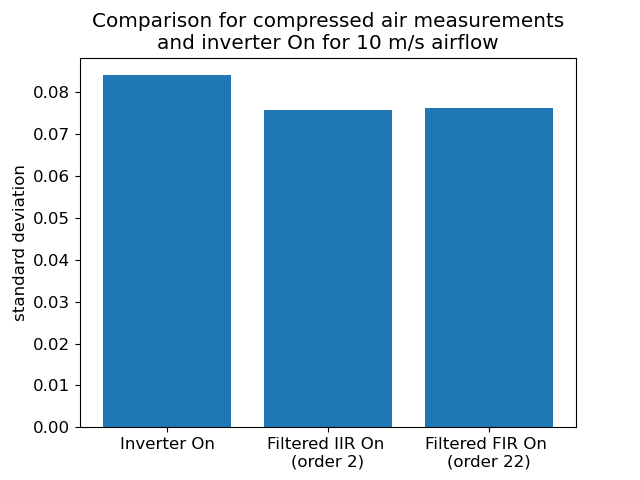
\includegraphics[scale=.7]{./src/test_std.png}}
\caption{Τυπική απόκλιση για ταχύτητα ανέμου \en{10\ m/s} συμπιεσμένου αέρα.}
\label{fig:ca-0-std}
\end{figure}

Ο έλεγχος των αποτελεσμάτων γίνεται με την χρήση της τυπικής απόκλισης. Κατά
την εφαρμογή οποιουδήποτε φίλτρου θα πρέπει η τυπική απόκλιση του σήματος να
μειώνεται, λογικό παράγωγο της διαδικασίας καθαρισμού σημάτων από θόρυβο, αφού
η απομάκρυνση από την διάμεση τιμή θα πρέπει να μειώνεται. Αν η τυπική απόκλιση
αυξάνεται, το σύστημα επηρεάζεται καταστρεπτικά από την διεργασία που
εφαρμόζεται σε αυτό. Παρατηρήθηκε αντίστοιχη συμπεριφορά αυξάνοντας την τάξη
του φίλτρου πέραν του αναγκαίου κατά πολλές τάξεις μεγέθους.

Στα διαγράμματα για την τυπική απόκλιση φαίνεται πως το φίλτρο \en{FIR}
πετυχαίνει καλύτερα αποτελέσματα αφού το σήμα εξόδου εμφανίζει μικρότερη τιμή
τυπικής απόκλιση του σήματος. Στην συνέχεια όμως θα δούμε πως το πλήθος των
τιμών που απέχουν κατά προκαθορισμένα διαστήματα από την διάμεση τιμή του σήματος
μειώνονται σημαντικά με την χρήση των \en{IIR}. Αυτό σημαίνει πως η δεύτερη
κατηγορία επηρεάζει με μεγαλύτερη ακρίβεια τις συχνότητες που βρίσκονται
αμέσως μετά την συχνότητα κατακρημνισμού.

Εδώ στην περίπτωση της αεροσήραγγας δεν κρίθηκε αναγκαίο να παρουσιαστεί
η τιμή των μετρήσεων με τον μετασχηματιστή κλειστό καθως το εν λόγω σήμα
καταγράφηκε για λόγους επιβεβαίωσης της εγκατάστασης και όχι για την μελέτη
της επιρροής του θορύβου.

\begin{figure}[h]
\centerline{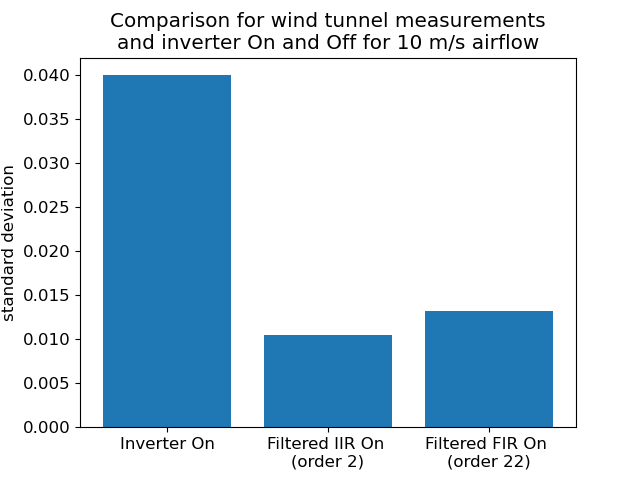
\includegraphics[scale=.7]{./src/std_wt_new.png}}
\caption{Τυπική απόκλιση για ταχύτητα ανέμου \en{10\ m/s} αεροσήραγγας.}
\label{fig:wt-0-std}
\end{figure}

Ένας δεύτερος τρόπος ελέγχου της διαδικασίας απόρριψης θορύβου περιλαμβάνει
την σύγκριση του ποσού των δειγμάτων που αποκλίνουν από την διάμεση τιμή στα
σήματα εισόδου και εξόδου του φίλτρου. Με αυτόν τον τρόπο μπορούμε να
συμπεράνουμε αν η πλειοψηφία των δειγμάτων αποτελούν τον θόρυβο ή όχι.
Αποτέλεσμα αυτού είναι πως ο θόρυβος είναι υψίσυχνος, αν μειώνοντας την
συχνότητα δειγματοληψίας μειώνεται και ο θόρυβος, αλλά διατηρείται η
πληροφορία που επιθυμούμε να καταγράψουμε δηλαδή δεν μεταβάλλεται σε μεγάλο
βαθμό η διάμεση τιμή του σήματος. Στην συνέχεια θα παρατεθούν αντίστοιχα
διαγράμματα για ταχύτητα πέντε μέτρα ανά δευτερόλεπτο, για τον
πεπιεσμένο αέρα σε σχέση με την αεροσήραγγα.

Για τα επόμενα διαγράμματα θα χρειαστεί να παρατεθούν κάποιες παράμετροι για
την κατανόησή τους. Η διακεκομμένη πράσινη γραμμή στην μέση του ορθογωνίου
παραλληλογράμμου ορίζει την διάμεση τιμή του σήματος. Το περίγραμμα του
παραλληλογράμμου εκφράζει το 75\% των δειγμάτων του σήματος και την διαφορά τους
από την διάμεση τιμή του δείγματος (σήμα). Τα ακρά αντιπροσωπεύουν την
μέγιστη και ελάχιστη τιμή που καταγράφεται σε ολόκληρο το δείγμα. Το υπόλοιπο
25\% του δείγματος βρίσκεται ανάμεσα στις ακραίες τιμές και το περίγραμμα. Έτσι
μπορούμε να προσδιορίσουμε την ποσότητα των δειγμάτων που περιέχουν την
πληροφορία της ταχύτητας του ανέμου, καθώς και αν κάποια διεργασία στο σήμα
το επηρέασε καταστρεπτικά.

\begin{figure}[t]
\centerline{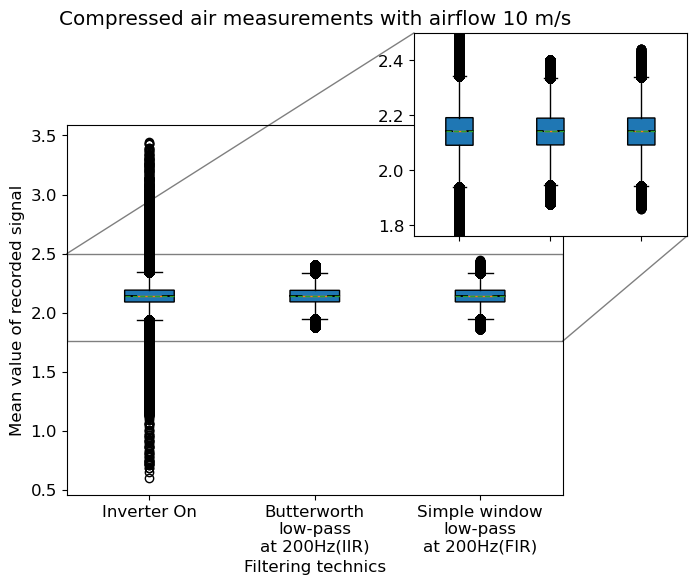
\includegraphics[scale=.6]{./src/whiskr_ca.png}}
\caption{Διάμεση τιμή για ταχύτητα ανέμου \en{10\ m/s} συμπιεσμένου αέρα.}
\label{fig:ca-0-mean}
\end{figure}

\begin{figure}[H]
\centerline{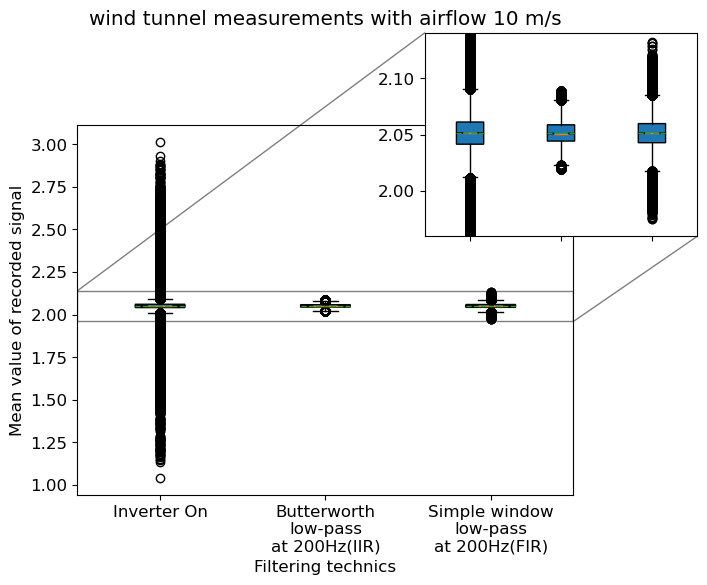
\includegraphics[scale=.6]{./src/whiskr.png}}
\caption{Διάμεση τιμή για ταχύτητα ανέμου \en{10\ m/s} αεροσήραγγας.}
\label{fig:ca-0-mean}
\end{figure}
Οι μετρήσεις με τον πεπιεσμένο αέρα φαίνεται να διατηρούν την διακύμανση από
την διάμεση τιμή του σήματος σχεδόν αμετάβλητη. Αίτιο της συμπεριφοράς αυτής
λογικά αποτελεί η μεγαλύτερη συχνότητα καταγραφής, καθώς προστείθεται μεγάλη
ποσότητα δειγμάτων από τα 100 στα 500 \en{kHz}. Εδώ όμως φαίνεται και το προσόν
των \en{IIR} φίλτρων.

Θα προσέξει κανείς πως, ενώ η τυπική απόκλιση του σήματος
μετά την εφαρμογή του \en{butterworth} είναι μεγαλύτερη από εκείνη για το \en{FIR}, το
αντίθετο συμβαίνει με την απόκλιση από την διάμεση τιμή. Αυτό συμβαίνει αφού
τα \en{IIR} συστήματα αποφέρουν πιο αναλυτικά αποτελέσματα και έχουν την
δυνατότητα για ακριβέστερο έλεγχο του εύρους των συχνοτήτων στην έξοδό τους.
\clearpage
\section{Αποτελέσματα καταγραφής και επεξεργασίας}
\label{sec:orgd0b90b9}
\subsection{Επεξεργασία δεδομένων ανέμου}
\label{sec:org1f69957}
Όπως φαίνεται και στο παραπάνω διάγραμμα ροής, για την ικανοποιητική σύγκριση
της επιρροής του φίλτρου στο σήμα που καταγράφηκε από τον αισθητήρα μέτρησης
της ταχύτητας ανέμου, προέχει ο έλεγχος της αλλοίωσης λόγω ανεπαρκούς
συχνότητας καταγραφής της κάρτας ΝΙ (\en{National\ Instruments}). Ο τρόπος που
επιλέχθηκε εδώ, ήταν η χρήση της τυπικής απόκλισης της κυματομορφής και να
ελεγχθεί η τυχών αύξησή της μετά την επεξεργασία. Από την αρχή μπορούμε να
παρατηρήσουμε πως ο μετασχηματιστής ευθύνεται για τις παρεμβολές,
και είναι εμφανής η αύξηση της τυπικής απόκλισης κατά 2 τάξεις μεγέθους. Επίσης
κατά την διαδικασία βελτιστοποίησης της τάξης του φίλτρου, λόγω βασικών
διαφορών στα \en{FIR} και \en{IIR} συστήματα, χρησιμοποιήθηκε διαφορετική αλλά παρόμοια
τιμή για την τάξη μεγέθους, ώστε να αποφευχθεί η κατασκευή διαγραμμάτων κάθε
φορά που πειραματιζόμασταν με διάφορα χαρακτηριστικά του εκάστοτε φίλτρου.

\begin{table}[htbp]
\caption{\label{std_1st}Πίνακας τυπικής απόκλισης σημάτων καταγεγραμμένα με διαφορετική παροχή ανέμου (συμπιεσμένος και μή).}
\centering
\begin{tabular}{lllrl}
 & Συμπιεσμένος αέρας &  & Αεροσήραγγα & \\
\hline
Μετ/στής & \en{On} & \en{Off} & \en{On} & \en{Off}\\
\hline
ταχ.=0 \en{m/s} & 0.0364 & 0.0062 & 0.0392 & 0.0076\\
ταχ.=5 \en{m/s} & 0.0434 & 0.0244 & 0.0385 & -\\
ταχ.=10 \en{m/s} & 0.0841 & 0.0763 & 0.0400 & -\\
ταχ.=15 \en{m/s} & - & - & 0.0421 & -\\
ταχ.=20 \en{m/s} & - & - & 0.0566 & -\\
\end{tabular}
\end{table}
\subsection{Εφαρμογή φίλτρων}
\label{sec:orgace62b8}
Για την παρεμβολή που επηρεάζει το σήμα του αισθητήρα θα εφαρμοστεί ένα φίλτρο
διέλευσης χαμηλών συχνοτήτων. Είμαστε σε θέση να γνωρίζουμε πως οι χαμηλές
συχνότητες του σήματος εμπεριέχουν όλο το ποσό της πληροφορίας που αποτελεί
την μέτρηση. Οι μετρήσεις που καταγράφηκαν για μηδενικές ταχύτητες, με τον
μετασχηματιστή κλειστό και ανοιχτό, χρησιμοποιήθηκαν για να βρεθεί η
ονομαστική τάση του αισθητήρα. Όσο για την επιλογή του κατάλληλου φίλτρου,
ως καταλληλότερα κρίθηκαν το \en{butterworth} από την κατηγορία των \en{IIR} για την
ελάχιστη διαστρέβλωση που αποφέρει κατά την εφαρμογή του στις συχνότητες
διέλευσης. Για την εύκολη σύγκριση των δύο μεθόδων, η έξοδος των φίλτρων
\en{FIR} έπρεπε να μετατραπούν από την μορφή της εξίσωσης μεταφοράς σε δευτέρας
τάξης “κομμάτια” (\en{sos\ output}) της αναπαράστασης της εξίσωσης μεταφοράς που
χαρακτηρίζει το φίλτρο. Για τις κατηγορίες που θα δούμε παρακάτω, οι βασικοί
τύποι των \en{FIR} φίλτρων που θα παρουσιαστούν, αναφέρονται στην ευρύτερη
βιβλιογραφία ως τύπου \en{I} και τύπου \en{II}. Η διαφορά είναι πως τα πρώτα παρουσιάζουν
θετική συμμετρία και έχουν τάξη ακέραιου περιττού αριθμού. Τα τύπου \en{II}
εμφανίζουν την ίδια συμμετρία, όμως η τάξη του φίλτρου είναι άρτιος αριθμός.

Υπάρχουν άλλες δύο κατηγορίες που εμφανίζουν αρνητική συμμετρία, όμως η
διαφορά στις τάξεις των φίλτρων τύπου \en{III,\ IV} είναι ανάλογες με των προηγούμενων
δύο τύπων.

Στην παρούσα εργασία ασχοληθήκαμε μόνο με φίλτρα από τους πρώτους 2 τύπους,
όμως αργότερα θα μπορούσαν να ερευνηθούν και περισσότεροι τύποι και
κατηγορίες παραθύρων. Όλες οι παραπάνω κατηγορίες συμπεριλαμβανομένων και
των \en{IIR}, στην έξοδό τους, το σήμα παραμορφώνεται εμφανίζοντας διαφορά φάσης
με το σήμα εξόδου. Έτσι, όπως αναφέρθηκε και νωρίτερα στην ενότητα 6.3,
επιλέγοντας την σωστή συνάρτηση από την κατάλληλη βιβλιοθήκη μπορούμε να
μειώσουμε το σφάλμα της αλλοίωσης και την πρόσθεση διαφοράς φάσης, σε
αποδεκτό βαθμό. Στην συνέχεια θα συγκριθούν τα διαγράμματα της πυκνότητας
ισχύος του σήματος με την μέθοδο του \en{Welch}, ώστε να εκλεγεί το κατάλληλο
προς εφαρμογή φίλτρο.
\subsection{Αποτελέσματα επεξεργασίας}
\label{sec:org33d97f4}
Για κάθε σήμα που καταγράφηκε εφαρμόστηκαν οι δύο από τις τρείς μεθόδους και
φάνηκε πως, ενώ για τα φίλτρα \en{IIR} είχαμε αποδεκτό βαθμό αλλοίωσης, ελέγχοντας την τυπική απόκλιση του σήματος εξόδου με εκείνη της εισόδου, τα \en{FIR}
φίλτρα παρέχουν καλύτερα αποτελέσματα. Ο τύπος του θορύβου που επηρεάζει το
σήμα του αισθητήρα, εμφανίζεται κυρίως σε συχνότητες που καταλαμβάνουν
ηλεκτρομαγνητικά κύματα ξεκινώντας από την περιοχή των 10-100 \en{kHz}.
Καταγράφηκαν και σήματα με συχνότητα δειγματοληψίας 500 \en{kHz} και ο θόρυβος
παραμένει, επομένως κρίθηκε πως πρόκειται για παρεμβολή μεγαλύτερης συχνότητας
από τις δυνατότητες καταγραφής του συστήματος που διαθέτουμε.
\subsubsection{Απομείωση θορύβου}
\label{sec:orge5e9e68}
Για την επιλογή του κατάλληλου φίλτρου εξετάστηκαν οι δύο βασικές
κατηγορίες, συγκρίνοντας την τιμή της τυπικής απόκλισης του σήματος, πριν
και μετά την εφαρμογή.  Από τους σημαντικότερους παράγοντες
που επηρεάζουν τον χρόνο υπολογισμού στα φίλτρα είναι η τάξη τους, δηλαδή
το πλήθος των συντελεστών του πολυωνύμου που θα κατασκευαστεί από τον
εκάστοτε αλγόριθμο. Όπως θα δειχθεί και στη συνέχεια, τα φίλτρα \en{IIR}, ενώ
αποδίδουν καλύτερα στην απομείωση του θορύβου με μικρότερης τάξης φίλτρα
από τα \en{FIR}, απαιτούν μεγαλύτερη υπολογιστική ισχύ λόγω της αναδρομικής
συμπεριφοράς τους. Στην πράξη ανάλογα με την συχνότητα καταγραφής και
την διάρκεια του σήματος, δηλαδή την ποσότητα των στοιχείων που εκφράζουν
το διακριτό σήμα προς επεξεργασία, επιλέγεται και μια από τις βασικές
κατηγορίες. Εδώ εξετάστηκαν και οι δύο μέθοδοι με σήματα διάρκειας περίπου
επτά δευτερόλεπτα σε συχνότητες καταγραφής 500 και 100 \en{kHz}. Η πηγή του
ανέμου από το καλώδιο πεπιεσμένου αέρα καταγράφηκε με συχνότητα 500 \en{kHz},
ενώ του ανεμιστήρα της αεροσήραγγας (\textbf{\en{ventilator}}) στα 100 \en{kHz}.

Όπως θα γίνει αντιληπτό στη συνέχεια, η διαδικασία παραγωγής των αποτελεσμάτων
αποτέλεσε το μικρότερο μέρος της εργασίας. Σημαντικό ήταν να καθοριστεί ο
τρόπος και οι μέθοδοι που θα χρησιμοποιηθούν και έπειτα να εφαρμοστούν
σωστά. Τέλος, θα δειχθεί πως και οι δύο μέθοδοι είναι αποδεκτοί για την
συγκεκριμένη εφαρμογή, υπό προϋποθέσεις που θα συζητηθούν στα συμπεράσματα.
\subsubsection{Διαγράμματα πυκνότητας ισχύος εισόδου και εξόδου φίλτρων}
\label{sec:orgb742b7e}
Η βασική ανάλυση των σημάτων γίνεται στο πεδίο των συχνοτήτων και κυρίως
μέσω της μεθόδου \en{Welch}. Αυτό συμβαίνει
καθώς απεικονίζοντας το σήμα στο πεδίο του χρόνου, εκτός της μεταβολής της
ισχύος του σήματος (αν αυτή απεικονίζεται), δεν μπορούμε να καθορίσουμε
τυχών θορυβώδη φάσματα συχνοτήτων. Έτσι πρώτο βήμα είναι να αποτυπωθεί το
φάσμα που επηρεάζει τις χαμηλές συχνότητες, όπου και καταγράφεται η
πληροφορία από τον αισθητήρα. Στις περισσότερες συσκευές οι συχνότητες
που ξεπερνούν τα \en{2-5\ kHz}, είτε αναφέρονται σε σήμα ήχου ή/και εικόνας,
είτε αποτελούν θόρυβο από το περιβάλλον πέραν εξαιρέσεων. Στην περίπτωση
που εξετάστηκε στο εργαστήριο, κρίθηκε πως μετά τα \en{2\ kHz}, το σήμα δεν
περιείχε “ουσιώδη” πληροφορία. Έτσι τα φίλτρα που εφαρμόστηκαν ήταν διέλευσης
χαμηλών συχνοτήτων από \en{100-2000\ Hz}.  Στα παρακάτω διαγράμματα σημειώνεται
με μπλε διακεκομμένη γραμμή.

Θα φανεί από τα πρώτα διαγράμματα πως τα \en{FIR} συστήματα παρουσιάζουν πολύ
πιο απότομη κλίση. Αυτό συμβαίνει καθώς ο κύριος παράγοντας που την επηρεάζει,
είναι η τάξη του φίλτρου. Όμως ταυτόχρονα αυξάνεται και η ταχύτητα υπολογισμού
αφού δεν καλείται αναδρομικά η έξοδος του φίλτρου όπως έχει σημειωθεί στην
ενότητα των φίλτρων. Κατά την εφαρμογή των δύο μεθόδων θα διαπιστώσουμε πως τα
αποτελέσματα αποκλίνουν σε πολύ μικρό βαθμό συγκρίνοντας τις τυπικές
αποκλίσεις των εξόδων σχετικά με την είσοδο των φίλτρων.

\begin{figure}[htbp]
\centering
\includegraphics[width=.9\linewidth]{./.ob-jupyter/d360114926b2d90b0427d6fb661e8048cb2de979.png}
\caption{\label{fc1_5}Διάγραμμα πεπιεσμένου αέρα για ταχύτητα ανέμου 5 \en{m/s} για φίλτρο \en{FIR}.}
\end{figure}


\begin{figure}[htbp]
\centering
\includegraphics[width=.9\linewidth]{./.ob-jupyter/41770b340e31d82fb61aa438d6db9b00da6dc74b.png}
\caption{\label{fc1_10_ref}Διάγραμμα πεπιεσμένου αέρα για ταχύτητα ανέμου 10 \en{m/s} για φίλτρο \en{FIR}.}
\end{figure}

\begin{figure}[htbp]
\centering
\includegraphics[width=.9\linewidth]{./.ob-jupyter/8927c062f57db4d1dca94ae8f1d157a38de6436f.png}
\caption{\label{ic1_5}Διάγραμμα πεπιεσμένου αέρα για ταχύτητα ανέμου 5 \en{m/s} για φίλτρο \en{IIR}.}
\end{figure}

\begin{figure}[H]
\centering
\includegraphics[width=.9\linewidth]{./.ob-jupyter/19fd61a7646c9dea2f7c4b030d5f7abd8d267a66.png}
\caption{\label{ic1_10}Διάγραμμα πεπιεσμένου αέρα για ταχύτητα ανέμου 10 \en{m/s} για φίλτρο \en{IIR}.}
\end{figure}

Στα επόμενα διαγράμματα θα παρατηρήσει κανείς πως ο θόρυβος είναι λιγότερο εμφανής από τα
προηγούμενα. Αυτό συμβαίνει λόγω της χαμηλότερης συχνότητας
καταγραφής στην περίπτωση της αεροσήραγγας. Όπως αναγράφεται και στους
τίτλους των διαγραμμάτων, τα παρακάτω σήματα καταγράφηκαν με συχνότητα
\en{100\ kHz}. Έτσι λόγω του θεωρήματος \en{Nyquist} το μέγιστο φάσμα που
μπορούμε να απεικονίσουμε υποχωρεί από τα \en{250\ kHz}, του πειράματος με
τον πεπιεσμένο αέρα, στα \en{50\ kHz}. Επιλέξαμε την μείωση αυτή, για
λόγους πειραματισμού καθώς η μείωση του αριθμού των δειγμάτων, προσφέρει
ταχύτερη επεξεργασία.
\begin{figure}[b]
\centering
\includegraphics[width=.9\linewidth]{./.ob-jupyter/83365afe07e883973c6e89a6dd65a0061e1b5c77.png}
\caption{\label{fi1_5}Σήμα αεροσήραγγας για ταχύτητα ανέμου 5 \en{m/s} για φίλτρο \en{FIR}.}
\end{figure}

\begin{figure}[htbp]
\centering
\includegraphics[width=.9\linewidth]{./.ob-jupyter/15f5bf879b541e5bc1b73e0332c602bd74453103.png}
\caption{\label{fi1_10}Σήμα αεροσήραγγας για ταχύτητα ανέμου 10 \en{m/s} για φίλτρο \en{FIR}.}
\end{figure}

\begin{figure}[htbp]
\centering
\includegraphics[width=.9\linewidth]{./.ob-jupyter/6594ff5fd31dd69a1536af30301d1aac417202d2.png}
\caption{\label{fi1_15}Σήμα αεροσήραγγας για ταχύτητα ανέμου 15 \en{m/s} για φίλτρο \en{FIR}.}
\end{figure}

\begin{figure}[htbp]
\centering
\includegraphics[width=.9\linewidth]{./.ob-jupyter/64249b5c4157e90451108bb9879becc15c03b362.png}
\caption{\label{fi1_w20}Σήμα αεροσήραγγας για ταχύτητα ανέμου 20 \en{m/s} για φίλτρο \en{FIR}.}
\end{figure}

\begin{figure}[htbp]
\centering
\includegraphics[width=.9\linewidth]{./.ob-jupyter/413d4b3af29809c7c97a35720ca06a57f28a9016.png}
\caption{\label{ii1_w5}Σήμα αεροσήραγγας για ταχύτητα ανέμου 5 \en{m/s} για φίλτρο \en{IIR}.}
\end{figure}

\begin{figure}[htbp]
\centering
\includegraphics[width=.9\linewidth]{./.ob-jupyter/4bbb618363e49a9aac8ae39296a0ff4261d46743.png}
\caption{\label{ii1_w10}Σήμα αεροσήραγγας για ταχύτητα ανέμου 10 \en{m/s} για φίλτρο \en{IIR}.}
\end{figure}

\begin{figure}[htbp]
\centering
\includegraphics[width=.9\linewidth]{./.ob-jupyter/e8940d740275ec8ca630ae50486acaf1f99469ea.png}
\caption{\label{ii1_w15}Σήμα αεροσήραγγας για ταχύτητα ανέμου 15 \en{m/s} για φίλτρο \en{IIR}.}
\end{figure}

\begin{figure}[htbp]
\centering
\includegraphics[width=.9\linewidth]{./.ob-jupyter/3c91e56ebb0cbafd43a170786a1f2a6298497fe8.png}
\caption{\label{ii1_w20}Σήμα αεροσήραγγας για ταχύτητα ανέμου 20 \en{m/s} για φίλτρο \en{IIR}.}
\end{figure}

\clearpage
\section{Σύγκριση αποτελεσμάτων}
\label{sec:org32a7fa2}
\subsection{Επιρροή μετασχηματιστή στον αισθητήρα}
\label{sec:orgbce3263}
Όπως θα γίνει αντιληπτό παρακάτω, απεικονίζοντας τις μετρήσεις για τον
μετασχηματιστή ανοιχτό και κλειστό σε αντίστοιχες ταχύτητες ανέμου, μπορούμε
να συμπεράνουμε δύο βασικά χαρακτηριστικά. Το πρώτο αναφέρεται στο εύρος των
συχνοτήτων που επηρεάζονται. Καθώς μειώνεται η συχνότητα καταγραφής, ο θόρυβος
των ηλεκτρομαγνητικών κυμάτων μεταφέρεται από τις υψηλές προς τις χαμηλές
συχνότητες. Λογικά το εύρος συχνοτήτων που καλύπτει ο θόρυβος βρίσκεται σε
μεγαλύτερες συχνότητες και επηρεάζεται από αλλοίωση, αφού η συχνότητα
καταγραφής είναι μικρότερη εκείνης του θορύβου.
\begin{figure}[H]
\centering
\includegraphics[width=.9\linewidth]{./.ob-jupyter/331fa0544fd4eee1883d71395b057362262efaff.png}
\caption{\label{fig:invOpenZero}Σύγκριση σήματος για μηδενική ταχύτητα και τον μετ/στή ανοιχτό και κλειστό καταγεγραμμένο στα \en{500\ kHz}.}
\end{figure}

\begin{figure}[H]
\centering
\includegraphics[width=.9\linewidth]{./.ob-jupyter/9bfbd4e78f07f15965a27406cbce9aae04380560.png}
\caption{\label{fig:invOpenZero100Ref}Σύγκριση σήματος αεροσήραγγας για μηδενική ταχύτητα και τον μετ/στή ανοιχτό και κλειστό καταγεγραμμένο στα \en{100\ kHz}.}
\end{figure}

Στις εικόνες \ref{fig:invOpenZero} και \ref{fig:invOpenZero100Ref} φαίνεται ο θόρυβος να μεταφέρεται από τα
\en{10-100\ kHz}
στα \en{1-10\ kHz}. Στο επόμενο
διάγραμμα (\ref{fig:invOpenTenRef}) φαίνεται η αύξηση της ισχύος του σήματος όταν ο
μετασχηματιστής είναι ανοιχτός. Πίο συγκεκριμένα παρατηρείται, μικρή αύξηση
της έντασης στην περιοχή των \en{200-800\ Hz}
με την έντονη αύξηση να παρουσιάζεται μετά τα \en{2-3\ kHz}
\selectlanguage{greek}. Η διαφορά αυτή είναι ξεκάθαρη και επηρεάζει το εύρος
που περιέχει την πληροφορία της ταχύτητας του ανέμου.


\begin{figure}[H]
\centering
\includegraphics[width=.9\linewidth]{./.ob-jupyter/3f25b84382916cfc87856e530afd82797c87e969.png}
\caption{\label{fig:invOpenTenRef}Σύγκριση σήματος για ταχύτητα 10 \en{m/s} και τον μετ/στή ανοιχτό και κλειστό.}
\end{figure}

\begin{figure}[H]
\centering
\includegraphics[width=.9\linewidth]{./.ob-jupyter/1a10efb47c09977de3d3265d2df849d41f8f40a8.png}
\caption{\label{fig:sfreqComp}Σύγκριση σήματος σε διαφορετικές συχνότητες καταγραφής με τον μετασχηματιστή ανοιχτό και μηδενική ταχύτητα ανέμου.}
\end{figure}

Στο σχήμα \ref{fig:sfreqComp} φαίνεται η επιρροή της μεταβολής συχνότητας καταγραφής
από επιλογή μέσω του λογισμικού.
\subsection{Αποδεκατισμός σήματος}
\label{sec:org87e4662}
\label{sec:decimation-chapter}
Η τεχνική του αποδεκατισμού εφαρμόστηκε κυρίως στην αρχή της επεξεργασίας
για να ελεγχθεί η διαδικασία καταγραφής. Κατέστη αναγκαίο να μπορέσουμε
να διασταυρώσουμε τον βαθμό, που το αρχικό σήμα υπέστη αλλοίωση από την
καταγραφή του. Επίσης σημαντικό ήταν να διασφαλιστεί πως κάθε μέθοδος
απόρριψης συχνοτήτων, θα μπορούσε να εφαρμοστεί σε μειωμένο αριθμό
δειγμάτων. Λόγω υψηλής συχνότητας καταγραφής μετά τα δέκα δευτερόλεπτα
διάρκειας σήματος, για την ολοκλήρωση των διαδικασιών που εφαρμόζονται, θα
χρειαζόμασταν πολύ χρόνο. Στα παρακάτω διαγράμματα αποτυπώνεται ο τρόπος
που επηρεάζει το σήμα η διαδικασία αυτή.
\subsubsection{\textbf{Διαγράμματα αποδεκατισμού με και χωρίς αλλοίωση στο πεδίο των συχνοτήτων}}
\label{sec:org50b220e}
\begin{figure}[htbp]
\centering
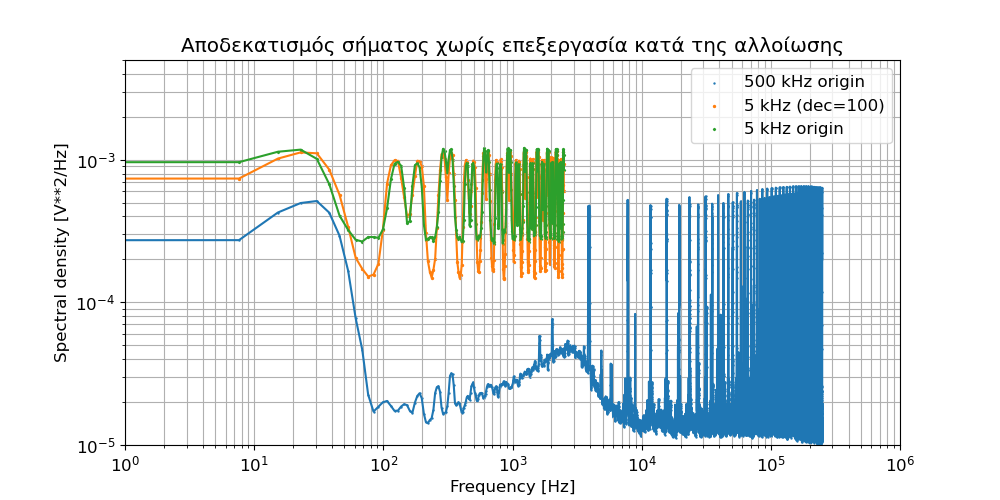
\includegraphics[width=500px,height=280px]{./decimation/with_aliasing.png}
\caption{\label{fig:with_al}Αποδεκατισμός σήματος χωρίς επεξεργασία κατά της αλλοίωσης για το σήμα του πεπιεσμένου αέρα με ταχύτητα ανέμου 0 \en{m/s} και μετ/στή ανοιχτό.}
\end{figure}

\begin{figure}[htbp]
\centering
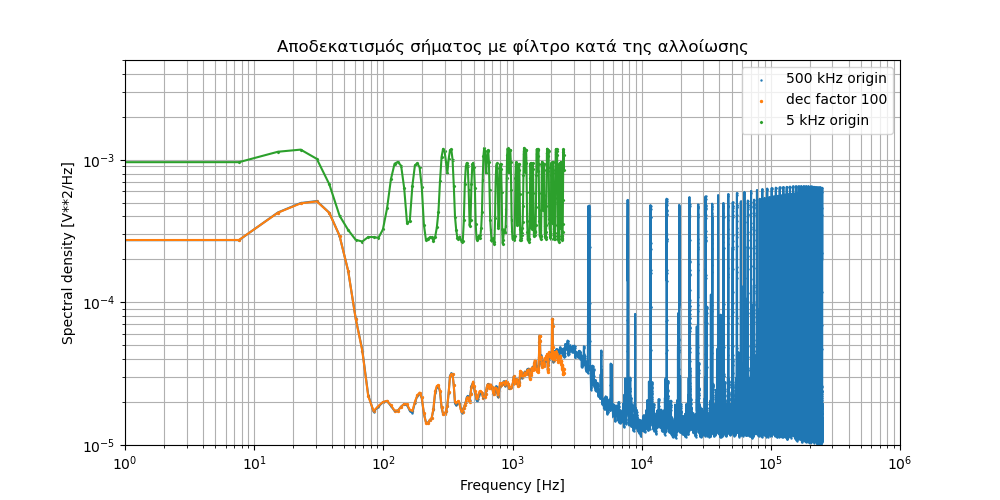
\includegraphics[width=500px,height=280px]{./decimation/anti_aliasing_fir.png}
\caption{\label{without_al}Αποδεκατισμός σήματος με φίλτρο \en{FIR} κατά της αλλοίωσης για το σήμα του πεπιεσμένου αέρα σε ταχύτητα ανέμου 0 \en{m/s} και μετ/στή ανοιχτό.}
\end{figure}

Όπως φαίνεται και παρακάτω, η διαδικασία της μείωσης του αριθμού των
δειγμάτων μπορεί να εντάξει αλλοίωση σε αρχικά “καθαρό” σήμα. Για να
μπορέσουμε να εφαρμόσουμε σωστά την συγκεκριμένη τεχνική, χρησιμοποιώντας
και κάποιο φίλτρο για την διόρθωση της αλλοίωσης, υπάρχουν πολλές μέθοδοι,
ήδη στις βιβλιοθήκες που χρησιμοποιήθηκαν για την ανάλυση των σημάτων.

\clearpage
\subsubsection{\textbf{Πίνακες επαλήθευσης μεθόδων στο πεδίο των συχνοτήτων}}
\label{sec:orgfb12b98}

Όπως φαίνεται παρακάτω, ο αριθμός των δειγμάτων καθώς
εφαρμόζουμε την μέθοδο του αποδεκατισμού παραμένει σταθερός, γεγονός που
καθορίζει την ορθότητα της εφαρμογής. Ο αριθμός δειγμάτων που παρατίθεται
μετρήθηκε μετά τον υπολογισμό της πυκνότητας ισχύος του σήματος και μόνο
για την ταχύτητα αναφοράς (0 \en{m/s}) του πεπιεσμένου αέρα. Η επιλογή
ήταν σκόπιμη, καθώς στα 500 \en{kHz} εμπεριέχεται ο μεγαλύτερος αριθμός
δειγμάτων. Έτσι έχουμε την δυνατότητα να υποστηρίξουμε ότι, αφαιρώντας
δείγματα από το σήμα δεν διαφοροποιείται το αποτέλεσμα σχετικά με την
καταγραφή του σε αντίστοιχη συχνότητα καταγραφής. Αυτό αντικατοπτρίζεται
συγκρίνοντας τους πίνακες \ref{some_ref}, \ref{rec_low_fs_ref} και \ref{dec_fir_ref}. Στους
δύο πρώτους φαίνεται πως η μείωση των δειγμάτων αποφέρει όμοιο σήμα με
καταγραφή σε εφάμιλλη συχνότητα.

\begin{table}[htbp]
\caption{\label{some_ref}Αποδεκατισμένο σήμα από 500 \en{kHz} για σήμα του πεπιεσμένου αέρα για ταχύτητα 0 \en{m/s}}
\centering
\begin{tabular}{lrrr}
\hline
Αριθμός δειγμάτων & χωρίς αποδεκατισμό & ανά 10 & ανά 100\\
\hline
Συχνοτήτων & 32769 & 3277 & 328\\
Ισχύος & 32769 & 3277 & 328\\
\end{tabular}
\end{table}

\begin{table}[htbp]
\caption{\label{rec_low_fs_ref}Καταγεγραμμένο σήμα του πεπιεσμένου αέρα για 0 \en{m/s} σε μικρότερες συχνότητες}
\centering
\begin{tabular}{lrr}
Αριθμός δειγμάτων & 50 \en{kHz} & 5 \en{kHz}\\
\hline
Συχνοτήτων & 3277 & 328\\
Ισχύος & 3277 & 328\\
\end{tabular}
\end{table}

\begin{table}[htbp]
\caption{\label{dec_fir_ref}Αποδεκατισμός με φίλτρο κατά της αλλοίωσης τύπου \en{F.I.R.} για το ανωτέρω σήμα}
\centering
\begin{tabular}{lr}
Αριθμός δειγμάτων & 5 \en{kHz}\\
\hline
\hline
Συχνοτήτων & 328\\
Ισχύος & 328\\
\end{tabular}
\end{table}

Στον πίνακα \ref{dec_fir_ref} η διαδικασία του αποδεκατισμού συνδυάστηκε με
την εφαρμογή φίλτρου κατά της αλλοίωσης, συμπεριλαμβανόμενη στην εντολή
του αποδεκατισμού. Η χρήση του εν' λόγω φίλτρου οδηγεί σε πολύ καλά αποτελέσματα,
όπως δείχνουν και τα διαγράμματα, \ref{fig:with_al} και \ref{without_al} καθώς απομοιώνουν
όσες συχνότητες αλλοιώνονται από την διαδικασία του αποδεκατισμού.

\begin{table}[!b]
\caption{\label{dec_anti_aliased}Πίνακας τυπικής απόκλησης για το σήμα πεπιεσμένου αέρα με ταχύτητα 0 \en{m/s} αποδεκατισμένο με φίλτρο κατά της αλλοίωσης τύπου \en{F.I.R.}.}
\centering
\begin{tabular}{X[1lm]X[2lm]}
\toprule
 &  & \en{decimation} & \\
\midrule
\en{fs} & \en{recorded at origin} & \en{decimated with anti-aliasing} & \\
\midrule
\en{5 kHz} & 0.0350 & 0.0058 & \\
\en{50 kHz} & 0.0366 & 0.0105 & \\
\en{500 kHz} & 0.0364 & - & \\
\midrule
 & \en{filtering operations} & \en{ in respect to cutoff frequency} & \\
\midrule
\en{low-pass filter} & \en{2 kHz} & \en{200 Hz} & \\
\midrule
\en{butterworth IIR} & 0.0035 & 0.0029 & \\
\en{simple FIR} & 0.0054 & 0.0054 & \\
\bottomrule
\end{tabular}
\end{table}

\clearpage
Τέλος, στον πίνακα \ref{dec_anti_aliased}, παρατηρούμε πως η τυπική απόκλιση
του σήματος, παρουσιάζει σταθεροποίηση στην μέθοδο των \en{FIR} συστημάτων
ανεξαρτήτος της συχνότητας αποκοπής του. Είναι εύκολο να συμπεράνουμε πώς,
ο τύπος \en{IIR} είναι πίο ακριβής καθώς για την ίδια διαφορά στις συχνότητες
απόρριψης παρατηρείται περεταίρω μείωση του θορύβου. Αυτό συμβαίνει λόγω
της μεθόδου της αναδρομής που αναφέραμε στα θεωριτικά κεφάλαια. Μας δίνεται
λοιπόν η δυνατότητα να αφαιρούμε τις συχνότητες που καταστρέφουν το σήμα
με μεγαλύτερη ακρίβεια και επομένως να διαχωριστούν φάσματα που δεν απέχουν
πολύ μεταξύ τους.
\vfill
\section{Συμπεράσματα}
\label{sec:org50202ef}
Όπως αναφέρθηκε αρκετές φορές και οι δύο κατηγορίες φίλτρων αποφέρουν αποδεκτά
αποτελέσματα. Η σύγκριση μπορεί να γίνει λοιπόν στην ταχύτητα
υπολογισμού των εξόδων όμως, αυτή \textbf{εξαρτάται ισχυρά} από την ποσότητα των
δειγμάτων του σήματος που επιθυμούμε να επεξεργαστούμε. Έτσι κυρίαρχο
ρόλο στην επιλογή του φίλτρου λαμβάνει η συχνότητα δειγματοληψίας (\en{fs}) και η
χρονική περίοδος που θα θέλαμε να αναλύσουμε. Ταυτόχρονα την \en{fs} καθορίζει
και το μέγιστο φάσμα συχνοτήτων σήματος που θέλουμε να καταγράψουμε, λόγω του
θεωρήματος της δειγματοληψίας. Επομένως είναι εύλογο να προσαρμόζεται η
επιλογή του φίλτρου σε σχέση με τον τύπο θορύβου (φάσμα συχνοτήτων)
που προσπαθούμε να απορρίψουμε, την συχνότητα δειγματοληψίας και την χρονική
περίοδο καταγραφής. Στην εγκατάσταση που εξετάστηκε, λόγω έντονων Η/Μ
παρεμβολών, παρουσιάστηκε ήπιος θόρυβος σε φάσμα άνω των \en{3-5\ kHz} με εμφανή
στοιχεία μετά τα \en{12\ kHz}. Λόγω της μεγάλης διαφοράς των φασμάτων θορύβου και
επιθυμητού σήματος, μπορούμε να χρησιμοποιήσουμε χωρίς πρόβλημα φίλτρα τύπου
\en{FIR} για την απόρριψη του. Η τυπική απόκλιση της εξόδου και των δύο τύπων
διαφέρουν σε αμελητέο βαθμό για την διάρκεια των επτά (7) δευτερολέπτων, του
σήματος, που επεξεργάστηκαν.

Μια ακόμα κύρια παράμετρος για την επιλογή αποτέλεσε η ποιότητα του σήματος
εξόδου, καθώς και η ακρίβεια του φάσματος διέλευσης συχνοτήτων που
προορίζονταν για επεξεργασία. Καταλήξαμε πως η επιθυμητή τιμή της τυπικής
απόκλισης του σήματος εξόδου θα εμφανίζει πτώση κατά μια τάξη μεγέθους
τουλάχιστον, σχετικά με την είσοδο του σήματος. Παρατηρούμε στους πίνακες της
προηγούμενης ενότητας ότι, εμφανίζεται σημαντική πτώση της τυπικής απόκλισης
για ταχύτητες μέχρι 5 \en{m/s} και όσο αυξάνεται η ταχύτητα του ανέμου η διαφορά
μειώνεται. Αυτό συμβαίνει λόγω της αύξησης της ισχύος του σήματος στις χαμηλές
συχνότητες, αφού ο θόρυβος παραμένει σταθερός και ο αισθητήρας μεταβάλει μόνο
τις χαμηλές συχνότητες κατά την καταγραφή. Η πληροφορία της
ταχύτητας του ανέμου παρέχεται σε συχνότητες έως \en{400\ Hz} από το αισθητήριο όργανο
με αποτέλεσμα να υπερκαλύπτεται, σε ισχύ, ο θόρυβος στις υψηλές ταχύτητες, όταν η
ταχύτητα του ανέμου ξεπερνά τα 10 \en{m/s}. Το συγκεκριμένο φαινόμενο μπορεί να
χρησιμοποιηθεί προς όφελος του ερευνητή, εφαρμόζοντας το ανάλογο φίλτρο μόνο
όταν καταγράφονται χαμηλές ταχύτητες ανέμου (ιδανικά \en\{0-10$\backslash$
m/s\}).
Σε υψηλότερες ταχύτητες, εφαρμόζοντας την τεχνική του αποδεκατισμού σε συνδυασμό
με ένα φίλτρο κατά της αλλοίωσης, όπως παρουσιάστηκε στο κεφάλαιο
\ref{sec:decimation-chapter}, δύναται να επιτύχουμε όμοια αποτελέσματα, αφού
μειώνοντας την συχνότητα καταγραφής, στην πράξη μειώνεται και το πλήθος των
δειγμάτων, άρα και το φάσμα συχνοτήτων που περιέχει θόρυβο στο αποδεκατισμένο σήμα.

Στην περίπτωση που απαιτείται λεπτομερή και αναλυτική απόρριψη φασμάτων
συχνοτήτων, προτείνεται ο συνδυασμός των δύο κατηγοριών φίλτρων. Αρχικά θα
πρέπει να εφαρμοστεί ο τύπος \en{FIR}. Έτσι απομειώνεται μεγάλο μέρος του θορύβου
σε υψηλές συχνότητες, μετά τα \en{5-8\ kHz} επιλέγοντας την συχνότητα αποκοπής στα
2 \en{kHz}, και στην συνέχεια με την εφαρμογή ενός \en{IIR} φίλτρου -λόγω μεγαλύτερης
ακρίβειας της δεύτερης κατηγορίας- να αποκτήσουμε πιο “καθαρό” σήμα τελικά στην
έξοδο. Συνδυάζοντας τις δύο κατηγορίες φίλτρων, αποφέρει μεν καλύτερα αποτελέσματα
όμως, αυξάνει σημαντικά τον χρόνο επεξεργασίας λόγος που συνιστάται μόνο σε
ειδικές περιπτώσεις ή/και μετά από σχετικές προϋποθέσεις του πειράματος. Η
συγκεκριμένη τεχνική δεν παρουσιάστηκε στην παρούσα εργασία γιατί κρίθηκε πολύ
χρονοβόρα.

Στόχος της παρούσας εργασίας ήταν ο πλήρης καθορισμός του θορύβου που
καταγράφηκε από τον αισθητήρα, η επιλογή κατάλληλου φίλτρου για την απόρριψη των
ανεπιθύμητων συχνοτήτων, όπως και η εύρεση της βέλτιστης μεθόδου ανάλογα την
εκάστοτε περίπτωση (ταχύτητα ανέμου, ποσότητα θορύβου, κ.α.). Για το μέλλον,
σημαντικές παράμετροι που δεν εξετάστηκαν πλήρως εδώ είναι η προέλευση καθώς και ο
καθορισμός της ισχύος και απόστασης της κάθε πηγής ηλεκτρομαγνητικών παρεμβολών
στον περιβάλλοντα χώρο. Μετά από υποθέσεις, καταλήξαμε πως υπάρχουν έτερες πηγές
Η/Μ κυμάτων που ενδέχεται να επηρεάζουν το καταγεγραμμένο σήμα. Εν κατακλείδι το
ποσό του θορύβου, ενώ ισχυρό, δεν καταστρέφει την πληροφορία της ταχύτητας του
ανέμου από το αισθητήριο όργανο και επομένως δεν υπάρχει ανάγκη εφαρμογής τεχνικών
επαναδημιουργίας του αρχικού σήματος και οι μέθοδοι του αποδεκατισμού και
φιλτραρίσματος κρίνονται επαρκείς.
\clearpage
\section{Βιβλιογραφία}
\label{sec:orgfb1110e}
\selectlanguage{english}
\noindent
A. J. Goldberg (1967). \emph{Vocoded speech in the absence of the laryngeal frequency}, Lexington, M.I.T..

\noindent
Edmund Lai (2003). \emph{Practical Digital Signal Processing}, Newnes.

\noindent
Heideman, M. and Johnson, D. and Burrus, C. (1984). \emph{Gauss and the history of the fast fourier transform}, IEEE ASSP Magazine.

\noindent
Ibrahim Abdulhadi Sulaiman and Hussain Mohammad Hassan and Mohammad Danish and Munendra Singh and P.K. Singh and Manisha Rajoriya (2022). \emph{Design, comparison and analysis of low pass FIR filter using window techniques method}, Materials Today: Proceedings.

\noindent
James W. Cooley and John W. Tukey (1965). \emph{{An algorithm for the machine calculation of complex Fourier series}}, Mathematics of Computation.

\noindent
Koichi Ichige and Naohisa Otsuka and Rokuya Ishii (1997). \emph{An automatic design procedure of IIR digital filters from an analog low-pass filter}, Signal Processing.

\noindent
McClellan, J.H. and Schafer, R.W. and Yoder, M.A. (2003). \emph{Signal Processing First}, Pearson/Prentice Hall.

\noindent
N. Agrawal and A. Kumar and Varun Bajaj and G.K. Singh (2021). \emph{Design of digital IIR filter: A research survey}, Applied Acoustics.

\noindent
Oppenheim, Alan V. and Schafer, Ronald W. and Buck, John R. (1999). \emph{Discrete-Time Signal Processing}, Prentice-hall Englewood Cliffs.

\noindent
Ryan B. Spelay and Kofi Freeman Adane and R. Sean Sanders and Robert J. Sumner and Randall G. Gillies (2015). \emph{The effect of low Reynolds number flows on pitot tube measurements}, Flow Measurement and Instrumentation.

\noindent
Steven W. Smith (2003). \emph{Continuous Signal Processing}, Newnes.

\noindent
Yong Moon Choi and Yoshiya Terao and Noboru Kurihara and Aya Iwai and Tatsuya Funaki and Woong Kang and Doan Trang Nguyen (2021). \emph{Revisit the Pitot static tubes in the standards}, Flow Measurement and Instrumentation.
\selectlanguage{greek}
\end{document}
